%% LyX 1.5.5 created this file.  For more info, see http://www.lyx.org/.
%% Do not edit unless you really know what you are doing.
\documentclass[a4paper,czech,czech,openright,cleardoubleempty,BCOR10mm,DIV11]{scrreprt}
\usepackage[T1]{fontenc}
\usepackage[utf8]{inputenc}
\usepackage{array}
\usepackage{longtable}
\usepackage{varioref}
\usepackage{wrapfig}
\usepackage{fancybox}
\usepackage{calc}
\usepackage{framed}
\usepackage{url}
\usepackage{graphicx}

\makeatletter

%%%%%%%%%%%%%%%%%%%%%%%%%%%%%% LyX specific LaTeX coěmmands.
\providecommand{\LyX}{L\kern-.1667em\lower.25em\hbox{Y}\kern-.125emX\@}
\newcommand{\lyxline}[1][1pt]{%
  \par\noindent%
  \rule[.5ex]{\linewidth}{#1}\par}
\newcommand{\noun}[1]{\textsc{#1}}
%% Special footnote code from the package 'stblftnt.sty'
%% Author: Robin Fairbairns -- Last revised Dec 13 1996
\let\SF@@footnote\footnote
\def\footnote{\ifx\protect\@typeset@protect
    \expandafter\SF@@footnote
  \else
    \expandafter\SF@gobble@opt
  \fi
}

\expandafter\def\csname SF@gobble@opt \endcsname{\@ifnextchar[%]
  \SF@gobble@twobracket
  \@gobble
}
\edef\SF@gobble@opt{\noexpand\protect
  \expandafter\noexpand\csname SF@gobble@opt \endcsname}
\def\SF@gobble@twobracket[#1]#2{}
%% Because html converters don't know tabularnewline
\providecommand{\tabularnewline}{\\}

%%%%%%%%%%%%%%%%%%%%%%%%%%%%%% Textclass specific LaTeX commands.
\newenvironment{lyxcode}
{\begin{list}{}{
\setlength{\rightmargin}{\leftmargin}
\setlength{\listparindent}{0pt}% needed for AMS classes
\raggedright
\setlength{\itemsep}{0pt}
\setlength{\parsep}{0pt}
\normalfont\ttfamily}%
 \item[]}
{\end{list}}

%%%%%%%%%%%%%%%%%%%%%%%%%%%%%% User specified LaTeX commands.
%<-------------------------------společná nastavení------------------------------>
\usepackage[czech]{babel}%počeštění názvů (Obsah, Kapitola, Literatura atp.)
\usepackage[]{hyperref} %odkazy v  pdf jsou klikací s barevnými rámečky
\usepackage[numbers,sort&compress]{natbib} %balíček pro citace literatury  
\usepackage{hypernat}%interakce mezi hyperref a natbib
\newcommand{\BibTeX}{{\sc Bib}\TeX}%BibTeX logo
\hypersetup{   % Nastavení polí PDF dokumentu 
pdftitle={NoSQL databáze},%   
pdfauthor={Jakub Josef},%  
pdfsubject={},%   
pdfkeywords={BigData, MongoDB, NoSQL, databases}%                             
}
\usepackage{multicol}




%<-----------------------------volání stylů----------------------------------------->
% (znak % je označení komentáře: co je za ním, není aktivní)
%<------------------------------------písmo----------------------------------------->
%\usepackage{packages/bc-latinmodern}
%\usepackage{packages/bc-times}
\usepackage{packages/bc-palatino}
%\usepackage{packages/bc-iwona}
%\usepackage{packages/bc-helvetika}


%<------------------------------záhlaví stránek------------------------------------>
%\usepackage{packages/bc-headings}
\usepackage{packages/bc-fancyhdr}

%<------------------------------hlavičky kapitol------------------------------------>
%\usepackage{packages/bc-neueskapitel}
%\usepackage{packages/bc-fancychap}

\makeatother

\usepackage{babel}

%java code block%

\usepackage{listings}
\usepackage{color}

\definecolor{dkgreen}{rgb}{0,0.6,0}
\definecolor{gray}{rgb}{0.5,0.5,0.5}
\definecolor{mauve}{rgb}{0.58,0,0.82}

% syntax highlight pro jazyk Java %
\lstset{,
  language=SQL,
  aboveskip=3mm,
  belowskip=3mm,
  showstringspaces=false,
  columns=flexible,
  inputencoding=utf8,
    extendedchars=true,
    literate=%
    {á}{{\'a}}1
    {č}{{\v{c}}}1
    {ď}{{\v{d}}}1
    {é}{{\'e}}1
    {ě}{{\v{e}}}1
    {í}{{\'i}}1
    {ň}{{\v{n}}}1
    {ó}{{\'o}}1
    {ř}{{\v{r}}}1
    {š}{{\v{s}}}1
    {ť}{{\v{t}}}1
    {ú}{{\'u}}1
    {ů}{{\r{u}}}1
    {ý}{{\'y}}1
    {ž}{{\v{z}}}1
    {Á}{{\'A}}1
    {Č}{{\v{C}}}1
    {Ď}{{\v{D}}}1
    {É}{{\'E}}1
    {Ě}{{\v{E}}}1
    {Í}{{\'I}}1
    {Ň}{{\v{N}}}1
    {Ó}{{\'O}}1
    {Ř}{{\v{R}}}1
    {Š}{{\v{S}}}1
    {Ť}{{\v{T}}}1
    {Ú}{{\'U}}1
    {Ů}{{\r{U}}}1
    {Ý}{{\'Y}}1
    {Ž}{{\v{Z}}}1,
  basicstyle={\small\ttfamily},
  xleftmargin=1cm,
  keywordstyle=\color{blue},
  commentstyle=\color{dkgreen},
  stringstyle=\color{mauve},
  breaklines=true,
  breakatwhitespace=true,
  tabsize=3
}
% vlastni package
\usepackage{placeins}
\usepackage{multirow}
% fonty popisku
\usepackage[font=small,labelfont=bf]{caption}
% radkovani 
\renewcommand{\baselinestretch}{1.2}
\renewcommand*{\lstlistingname}{Kód} %prejmenovani lstlisting
\renewcommand*{\lstlistlistingname}{Seznam ukázek kódu}
\begin{document}

\cleardoublepage{}~\thispagestyle{empty}\begin{center}\pagenumbering{roman}\vspace{10mm}


\textsf{\textsc{\noun{\LARGE Univerzita Hradec Králové}}}\\
\vspace{0.5em}
\textsc{\noun{\LARGE Fakulta informatiky a managementu}}\\
\vspace*{1em}
\textsf{\textsc{\noun{\Large katedra informatiky a kvantitativních metod }}}


%%% Aby vložení loga  správně fungovalo, je třeba mít soubor uhk.png nahraný v adresáři logo,
%%% tj. v adresáři, kde se nachází překládaný zdrojový soubor. 
\vspace{4cm}

\textsf{\huge BAKALÁŘSKÁ PRÁCE}{\huge \par}

\vspace{15mm}


\textsf{\LARGE NoSQL databáze}{\LARGE \par}

\vspace{10mm}


\end{center} 

\vspace*{\fill}


\vspace{10mm}


\begin{description}
\item [{{\large Autor:}}] \noindent \textsf{\large Jakub Josef}{\large \par}
\item [{{\large Vedoucí~práce:}}] \noindent \textsf{\large doc. Ing. Filip Malý, Ph.D.}{\large \hfill{}}\textsf{\large Hradec Králové, 2014}{\large{}
% doplňte rok vzniku vaší bakalářské práce
}{\large \par}
\end{description}

\clearpage{}
~\thispagestyle{empty}{\small ~\vfill{}
}{\small \par}

\noindent {\small \vfill{}
 % nastavuje dynamické umístění následujícího textu do spodní části stránky
~}{\small \par}

\noindent {\small Prohlašuji, že jsem bakalářskou práci vypracoval samostatně a uvedl jsem všechny použité prameny a literaturu.}{\small \par}

{\small \bigskip{}
}\noindent {\small{} Ve Smiřicích dne \today\hspace{\fill}Jakub Josef}\\
{\small{} % doplňte patřičné datum, jméno a příjmení
}{\small \par}

{\small %%%   Výtisk pak na tomto míste nezapomeňte PODEPSAT!
%%%                                         *********
}{\small \par}

\clearpage{}
~\thispagestyle{empty}{\small ~\vfill{}
}{\small \par}

\noindent {\small Děkuji doc. Ing. Filipu Malému, Ph.D. za odborné vedení bakalářské práce a poskytování rad. \newpage{}}{\small \par}
\clearpage{}
~\thispagestyle{empty}{\small ~\vfill{}
}{\small \par}
\noindent {\small \vfill{}
 % nastavuje dynamické umístění následujícího textu do spodní části stránky
~}{\small \par}
\section*{Anotace}
Tato práce se zabývá problematikou nerelačních databází, zvaných NoSQL databáze. Jedná se o nová databázová řešení, která se vzdávají některých vlastností tradičních SQL databází, jako jsou schémata nebo podpora transakcí. Místo toho nabízejí velmi vysokou rychlost zpracování a výborné možnosti škálování výkonu. Práce představí samotný pojem NoSQL a jeho hlavní zástupce, ale především si klade za cíl srovnat relační databázi MySQL s dokumentově orientovanou NoSQL databází MongoDB. Obě tyto databáze se totiž hodí pro nasazení ve webové aplikaci jako hlavní úložiště dat. Byly provedeny výkonnostní testy, které měly za úkol porovnat tyto databáze mezi sebou. Testy lze nalézt v praktické části. Závěrem práce jsou shrnuty výsledky měření a představeny další možnosti výzkumu v této oblasti.


\section*{Annotation}
Title: NoSQL databases
\vspace{0.5cm}

\noindent This bachelor thesis deals with new types of non-relational databases called NoSQL. This new database solutions are not support some traditional SQL features like schemas or transactions, but offer very high processing speed and great scalability. Thesis explains a whole term NoSQL with best knows databases of each type. But the main purpose is to compare relational database MySQL with document-oriented NoSQL database MongoDB, which can be used in the same place in web application, as a main data store. Results of performance testing of those databases, can be find in practical part. All results is summarized in conclusion. You can also find some good possibilities of next research in the last part.

\noindent {\small ~\vfill{}
}{\small \par}

\cleardoublepage{}\thispagestyle{empty}{\small \tableofcontents{}% vkládá automaticky generovaný obsah dokumentu
\cleardoublepage{}}{\small \par}

\pagenumbering{arabic}%start arabic pagination from 1 


\chapter{Úvod}Webové stránky nebo počítačové programy vznikají tak, že je určitý tým lidí naprogramuje v nějakém programovacím jazyce. To už je už prakticky součástí obecného povědomí široké veřejnosti. Avšak neméně důležitou součástí téměř každé aplikace, ať už se jedná o webovou stránku nebo desktopovou aplikaci, je databáze. To je způsob ukládání jakýchkoliv dat, která jsou nezbytná pro fungování aplikace jako celku. Nyní v době obrovského rozvoje a rozmachu propojení informačních technologií se životem obyčejného člověka se značně zvyšují nároky na tyto databáze. Každou sekundou na Internetu přibude obrovské množství dat, které je třeba někde ukládat a zároveň být schopen v nich velmi rychle orientovat. Proto se v posledních letech značně mění náhled na problematiku databázových systémů a můžeme pozorovat odklon od klasických aplikačně složitých SQL serverů k jednodušším řešením. Snížíme tedy složitost databáze,  abychom získali větší rychlost a škálovatelnost. Asi nejznámějším případem je příběh společnosti Facebook, která byla nucena kvůli obrovskému množství dat vytvořit zcela nový databázový systém \cite{cassandra}. Tento databázový systém nebyl založený na principu relačních databází, jednalo se tedy o jeden s prvních případů nasazení nerelační databáze do reálného provozu ve webové aplikaci.  Klasické, mnoho let používané SQL servery jsou typickým příkladem relačních databází, kde jednotlivé entity mají definovány relace na jiné, zatímco  nerelační databáze nic takového neznají a vzhledem k jejich fungování, ani nepotřebují. Jedním ze stěžejních výhod těchto řešení je absence entitového modelu, každá entita tedy může nést libovolné množství jakýchkoliv parametrů různých datových typů. Pro tyto nerelační aplikačně méně komplexní databázová řešení se vžil název NoSQL databáze a bude se jimi zabývat i tato práce.

\section{Cíl, metodika a předpoklady práce}
Hlavním cílem práce je porovnání SQL a NoSQL databází, rychlosti dotazování na jednotlivé databázové servery a představení možností migrace existujících aplikací běžících na klasických SQL serverech. Práce předpokládá základní znalosti z oblasti vývoje webových aplikací a je určena programátorům, kteří mají zájem o použití některé z NoSQL databází místo tradičního SQL řešení. Práce nejprve stručně popíše relační SQL databáze, poté zavede pojem NoSQL databáze, stručně představí aktuální stav v oblasti a existující databázové servery, jejich účel a hlavní výhody. V praktické části se práce zabývá porovnáním relačních SQL databází s novými moderními NoSQL databázemi. Databáze budou porovnávány z hlediska rychlosti zpracování pomocí výkonnostních testů. Testy se budou snažit simulovat situace podobné velmi vytíženým webovým aplikacím, jako je např. objednávka velkého počtu zákazníků najednou, nebo obsluha mnoha uživatelů. Kvůli dobrým možnostem škálování, které NoSQL databáze nabízejí, budou testy také spouštěny na větším počtu databázových serverů, v tzv. clusteru. Cluster bude provozován virtuálně pomocí virtualizační platformy VirtualBox na linuxovém operačním systému Ubuntu a jednotlivé databázové servery budou řešeny pomocí aplikačních kontajnerů Docker. Zároveň bude také otestován výkon databáze pouze na jednom samostatném serveru. Tento server bude provozován lokálně na Mac OS X. Dále budou databáze porovnány podle možností migrace ze zažitých SQL databázových serverů. Na základě těchto testů, bude rozhodnuto zda-li je NoSQL databáze MongoDB vhodnější pro použítí ve webové aplikaci, která by běžně nasadila relační databázi MySQL.

\vspace{0.5cm}
\noindent \emph{Technologie použité v práci:}
\begin{itemize}
\item VirtualBox: virtualizační platforma
\item Vagrant: open source správce virtuálních serverů
\item Ubuntu 12.04: operační systém databázových serverů
\item Docker: nástroj pro tvorbu aplikačních kontajnerů
\item MongoDB: dokumentové orientovaná NoSQL databáze
\item MySQL: open source relační SQL databáze
\item D3.js: framework pro práci s grafy
\item yED: nástroj na tvorbu diagramů a schémat
\end{itemize}

\section{Struktura práce}
Práce se fakticky dělí na dvě základní části. V teoretické části je čtenáři poskytnut lehký úvod do SQL, popsány principy klasických relačních databází a jejich dopady. Dále je v práci představeno NoSQL jako samotný pojem a popsány důvody jeho vzniku. Následuje rozdělení současných NoSQL databázových systémů podle způsobu zacházení s daty. Toto rozdělení se postupem času ustálilo jako to nejlepší. Jednotlivé skupiny databázových systému jsou popsány, je vysvětleno jejich zařazení a zachyceny největší výhody. Téměř každá z těchto skupin byla vytvořena účelně, jako řešení problémů na které relační databáze nestačily. Práce nejpodrobněji popisuje dokumentově orientovanou databázi MongoDB, o které se čtenář mnohé dozví v praktické části této práce. Cílem praktické části je totiž porovnat SQL databázi MySQL právě s MongoDB. V této části práce jsou stručně představeny MySQL a MongoDB servery, včetně ukázek instalace a provozu. Důležitým kritériem každého testování je popis testovacích dat a testovacího prostředí. Těmito dvěma kapitolami práce pokračuje až k samotnému testování. Zde jsou popsány jednotlivé testy, které by měli simulovat situace které v internetovém provozu reálně nastávají. Každý z těchto testů, byl pro srovnání spuštěn i ve virtuálním MongoDB databázovém clusteru. Závěrem práce shrne zjištěné výsledky a nabídne podněty k dalšímu bádání v této oblasti.

\section{Aktuální stav v oblasti NoSQL databází}
Podle aktuálních poznatků v oblasti výkonostních testů databázových serverů by NoSQL databáze, při malém počtu dat, neměly být zásadně rychlejší než klasické SQL databáze. Jejich hlavní síla tkví v jednoduchém škálování výkonu a schopnosti efektivně pracovat s velkým množstvím dat. Aplikačně nejméně komplexní řešení typu \emph{key - value úložišť} se již používají v reálném provozu pro obsluhu velkého počtu jednoduchých dat, například uživatelských sessions \footnote{Sezení uživatele, unikátní řetězec sloužící k identifikaci přihlášeného uživatele.}. Key-Value databáze Redis, vyznačující se velmi vysokou rychlostí zpracování, například dosahuje odezvy kolem 1-2ms při 50 aktivních uživatelích zároveň. Z 10000 požadavků se necelých 80\% zvládlo vyřídit během jedné milisekundy. Tohoto výsledku nebylo dosaženo na nějakém výkonném serveru, ale na obyčejném počítači s dvoujádrovým procesorem a operačním systémem Linux \cite{redisBenchmark}. Toto měření ukazuje, jak rychlá NoSQL databáze může být pokud je aplikačně velmi jednoduchá a dobře navržená. Redis je typickým zástupcem velmi jednoduchých databází, které v podstatě umí pouze uložit hodnotu s nějakým unikátním klíčem, a poté jí zase na jeho základě získat. Tato práce se bude primárně zabývat porovnáním NoSQL databáze MongoDB se SQL databází MySQL. MongoDB je zástupce dokumentově orientovaných databází a je tedy mnohem aplikačně komplexnější databází než již zmíněný Redis. Bývá vnímána jako nejlepší kompromis mezi výkonem a schopnostmi databázového serveru. Podle již provedených testů je několikanásobně rychlejší než MySQL, pokud pracujeme s velkým počtem záznamů (řádově statisíce až miliony) a chceme k nim přistupovat paralelně \cite{nosqlBenchmark}.

Tyto testy byly provedeny na jednom výkonném databázovém serveru a lze očekávat, že při použítí clusteru se výsledky ještě zlepší. Avšak hlavním účelem použití clusteru zůstává vysoká dostupnost a spolehlivost. Jednou z dalších výhod těchto nových technologických řešení je kvalitní návrh, který plně podporuje škálování. To znamená, že lze velmi dobře dynamicky reagovat na zvětšování uživatelské základny webové aplikace. Pokud nastane situace, kdy je databáze přetížená, stačí jednoduše zvýšit výkon clusteru přidáním dalších databových serverů. Teoreticky lze takto navyšovat rychlost a kapacitu databáze dokonečna. Horizontálně škálovatelný návrh je jednou z hlavních výhod NoSQL databází.

\begin{table}[h]
\centering
	\caption{Výkonostní testy MongoDB vs. MySQL \cite{nosqlBenchmark}}
    \begin{tabular}{ | l | l | l | p{5cm} |}
    \hline
    Databáze & Operace & Počet řádků & Čas odpovědi \\ \hline
    MySQL & Vložení dat & 10000000 & 1130493ms \\ \hline
    MongoDB & Vložení dat & 10000000 & 411121ms \\ \hline
    MySQL & Získání dat & 5000 & 66ms \\ \hline
    MongoDB & Získání dat & 5000 & 2ms \\ \hline
    MySQL & Získání dat & 500000 & 447ms \\ \hline
    MongoDB & Získání dat & 500000 & 3ms \\ \hline
    \end{tabular}
    \label{tab:mongoVsMySQLTests}
\end{table}

\section{Literární rešerše v oblasti}
NoSQL databáze jsou relativně mladou a zajímavou technologií, proto se jimi již zabývalo velké množství domácích i zahraničních vědců ve svých pracích. V České republice byl jedním z prvních Richard Günzl na Vysoké škole ekonomické v Praze, který se ve své práci věnoval hlavně obecné problematice NoSQL databází. Představil samotný pojem, nejznámější NoSQL databáze a používané datavé modely. Günzl také ukázal oblasti webové nebo desktopové aplikace, kde je výhodné NoSQL databáze nasazovat \cite{gunzl}. Velmi zajímavou prací, která defakto navazuje na práci Günzla, zpracoval Martin Petera také z VŠE Praha. Jeho práce se dopodrobna zabývá hlavně NoSQL databází MongoDB, popisuje způsob její instalace, obsluhy a implementaci v aplikacích. Je zde dobře popsán proces \emph{mongod}, který zajišťuje běh samotného MongoDB serveru, včetně všech jeho režimů a parametrů. Dále práce popisuje možnosti dotazování a zpracování výsledků nad touto databází \cite{peteraMongo}. V zahraničí se tématu věnoval například Christof Strauch z univerzity ve Stuttgartu, který na téma NoSQL databází zpracoval obsáhlou diplomovou práci. Práce rozebírá důvody vzniku NoSQL databází, jejich základní principy a modely ukládání dat. Poté rozebere tři základní oblasti těchto databází, key-value úložiště, sloupcově-orientované a dokumentové databáze. Práce popíše nejznámější databázové servery v každé z těchto oblastí. Tato práce ale vznikala již od roku 2010 a díky velmi rychlému a dynamickému vývoji v oblasti, obsahuje některé zastaralé nebo překonané pojmy nebo principy \cite{strauchNosql}. Další prací českého studenta je práce s prostým názvem \emph{NoSQL databáze} Tomáše Panyka z Jihočeské univerzity v Českých Budějovicích. Jeho práce kromě obvyklého představení NoSQL databází, porovnává MySQL s Redisem. Redis se jako zástupce úložišť typu klíč - hodnota v tomto porovnání ukázal jako nesrovnatelně rychlejší \cite{panykoNosql}. Tento výsledek se dal vzhledem k principům SQL očekávat a dle mého názoru jsou porovnávány nesprávně vybrané technologie. Redis a MySQL jsou totiž zacíleny na správu úplně odlišných typů dat. Porovnání, kterým se bude zabývat tato práce, tedy porovnání NoSQL databáze MongoDB s SQL databází MySQL se mi jeví přijatelnější, protože oblast jejich nasazení v aplikaci je velmi podobná.


\chapter{SQL Databáze a jejich princip}
SQL (Structured Query Language), jazyk pro získávání strukturovaných dat, vznikl z jazyka SEQUEL, který vynalezla společnost IBM v 70. letech minulého století jako jazyk sloužící z získání takzvaných relačně orientovaných dat. Inspirací byl jeden z prvních relačních modelů, zvaný "A Relational Model of Data for Large Shared Data Banks" \cite{coddSql}, jehož autorem je Edgar F. Codd.  Během let se relačně orientované databáze osvědčily a dnes jsou používány ve spoustě aplikací na celém světě. Pojem SQL se postupem času zažil jako pojmenování celého odvětví databázových serverů, postavených na stejném nebo velmi podobném principu relační správy dat.

SQL databáze jsou tedy typickém zástupcem relačních databází, kde základním prvkem je tzv. relace. Můžeme je definovat podle Jaromíra Skřivana jako množinu tabulek, které se skládají ze sloupců a řádků. Sloupce odpovídají jednotlivým vlastnostem (atributům) entity. Údaje v jednom řádku tabulky reprezentují právě jednu entitu.
Budu mít např. tabulku ZAMĚSTNANEC, která bude popisovat entitu pracovníka ve firmě. Sloupce tabulky budou: ČÍSLO, JMÉNO, PŘÍJMENÍ, DAT\_NAR, PLAT a SMLOUVA\_OD. Atribut DAT\_NAR značí datum narození pracovníka a SMLOUVA\_OD uvádí datum, od kterého je pracovník v naší firmě zaměstnán \cite{sqlDatabaze}. Představme si, že reálnému světu odpovídá následující naplnění tabulky.

\begin{figure}[h]
\begin{centering}
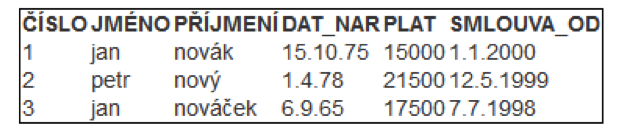
\includegraphics[scale=1]{obrazky/sql-tabulka}
\par\end{centering}
\caption{SQL Tabulka \cite{sqlDatabaze} \label{fig:sqlTable}}
\end{figure}


Data jsou tedy v databázi uspořádána do tabulek, kde každá tabulka má přesně daný počet sloupců, tabulka je tedy modelem uložení dat. 
K obsluze SQL databáze se používá speciální dotazovací jazyk SQL, který se podle Skřivana skládá z několika částí:
\begin{itemize}
\item Data Definition Language (DDL)
\item Storage Definition Language (SDL)
\item View Definition Language (VDL)
\item Data Manipulation Langugage (DML)
\end{itemize}
První částí jazyka SQL je jazyk DDL. Jedná se o jazyk pro vytváření databázových schémat a katalogů. Způsob ukládání dat v tabulkách definuje jazyk SDL. Třetí částí určenou pro návrhnáře a správce databází je jazyk VDL, který definuje databázové pohledy. Poslední částí je DML, jazyk popisující manipulaci s daty. Jeho součástí jsou známe příkazy INSERT, UPDATE, DELETE a nejpoužívanější příkaz SELECT \cite{sqlDatabaze}.

Relační SQL databáze jsou schopny pokrýt všechny typy vazeb, včetně vazby m:n, kterou je ale nutné implementovat pomocí vazebních tabulek \footnote{Tabulky nesoucí dvojice unikátních identifikátorů reprezentující relaci mezi dvěma entitami.}. Zároveň tyto databáze plně podporují cizí klíče. Mezi nejznámější SQL databázové servery patří MySQL, MSSQL, PosgreSQL nebo Oracle. MySQL je open source databázový server vyvinutý firmou Sun, dnes patřící společnosti Oracle. Tento databázový server je dostupný zdarma a je velmi oblíbený mezi vývojáři PHP webových aplikací. MSSQL je implementace SQL serveru od společnosti Microsoft, často používaná mezi vývojaři ASPX aplikací.
Většina z nich podporuje primární i sekundární indexování atributů, tedy je čistě na programátorovi nebo návrháři databáze, aby navrhl atributy, které bude vhodné indexovat a zrychlit tak odezvu databáze. Postupem času se tyto databáze vyvinuly a dnes nabízejí také možnosti pro ukládání souborů nebo geometrických dat.

\section{Princip ukládání dat}
SQL databáze typicky ukládají data do tabulek, které představují schéma (model) entit, v nich uložených. Jednotlivé atributy entity reprezentují sloupce tabulky, mají určitý datový typ například celé číslo, časový údaj nebo řetězec. Každému sloupci lze definovat jeho délku, což umožňuje velmi dobře omezit podobu ukládáných dat a zároveň šetřit diskový prostor databázového serveru. Některým sloupcům mohou být nastaveny výchozí hodnoty nebo být označeny jako nepovinné. Každý sloupec určený pro atribut typu řetězec, musí být nastavené kódování. Nepsaným standardem je pro tyto atributy používat UTF-8. \footnote{Způsob kódování řetězců podporující veškeré znaky národních abeced Unicode.} Jeden ze sloupců (zpravidla první), by měl být označen jako takzvaný \emph{primární klíč}. V tomto sloupci musí být uložen unikátní identifikátor řádku tabulky a databázový server poté sám kontroluje jedinečnost tohoto sloupce. Primární klíč může obsahovat uměle vytvořenou nebo přirozeně se vyskytující jedinečnou hodnotu, například rodné číslo. Struktura SQL tabulky je tedy předem daná a každá změna v ní musí být aplikována na všechny řádky, které obsahuje. To v praxi znamená, že přidání nebo odebrání sloupce v tabulce obsahující velké množství záznamů, představuje časově velice náročnou operaci \cite{mysqlDataTypes}.
Většina v současnosti používaných databázových serverů dobře podporuje indexování atributů, které primárně slouží k urychlení dotazování na tabulku. Index by měl být přidán na ty sloupce, u kterých se očekává časté použití v SQL dotazech. Indexy mohou být také použity k ověření jedinečnosti dat ve sloupci (tzv. unikátní index) nebo pro fulltextové vyhledávání.

\begin{figure}[h]
\begin{centering}
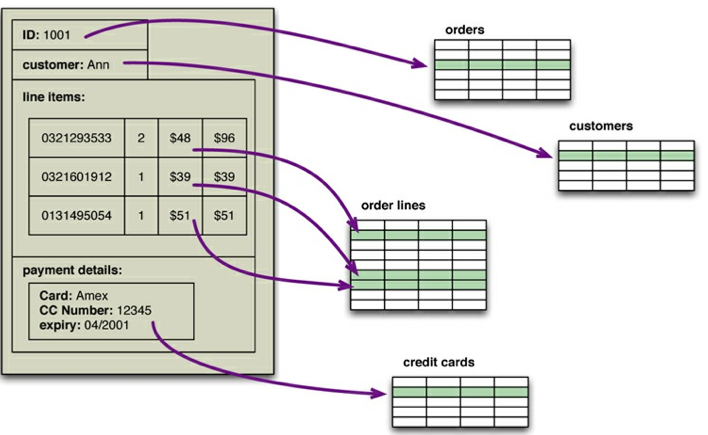
\includegraphics[scale=0.5]{obrazky/data2table}
\par\end{centering}
\caption{Ilustrace webového formuláře a potřebých datulek s daty \cite{nosqlDistilled} \label{fig:data2table}}
\end{figure}

Z principu relačních databází vyplývá, že pro zachycení složitějších vazeb nebo hierarchických dat je nutné použít velké množství tabulek. Vztah mezi zobrazením a reprezentací dat dobře ilustruje obrázek výše, jednoduché vztahy mezi objednávkou (tabulka orders) a zákazníkem (tabulka customers) jsou realizovány pomocí cizích klíčů. Na složitější vazby typu m:n je třeba vytvořit nové vazební tabulky (order lines), které slouží pouze tomuto účelu a nenesou žádná další data.

\vspace{0.5cm}
\noindent \emph{Některé datové typy v MySQL}
\begin{itemize}
\item INT, INTEGER - celé číslo, rozsah cca -2 až 2 milióny, existují varianty s větším rozsahem hodnot
\item FLOAT, DOUBLE - desetinné číslo
\item DATE, DATETIME, TIMESTAMP - reprezentace času
\item CHAR, VARCHAR, TEXT - řetězce
\item BLOB - binární data
\end{itemize}

\section{Integrita dat v SQL databázích}
Většina SQL serverů poskytuje záruky integrity dat, databázové operace se zpravidla provádějí v transakcích, které musí splňovat tzv. \emph{vlastnosti ACID} \cite{acid}.
\begin{itemize}
\item Atomic (atomičnost) - každá transakce musí být atomická, provedou se buď všechny změny v databází nebo žádná
\item Consistent (konzistence) - transakce představuje přechod z jednoho konzistentního stavu databáze do druhého
\item Isolated (izolace) - každá transakce je nezávislá a nemůže být ovlivněna ostatními transakcemi
\item Durable (trvanlivost) - pokud je transakce dokončena, změny, které provedla, jsou trvalé
\end{itemize}
Každá transakce představuje operaci provedenou uživatelem aplikace, tedy například objednávku z internetového obchodu nebo finanční operaci pracovníka pobočky v bankovním systému. Obsahuje všechny změny v tabulkách, které jsou pro daný úkon vzhledem k návrhu aplikace potřeba. Transakce fungují jako mechanismus ochrany před nekonzistencí databáze, poskytují záruky, že nedošlo k ztrátě nebo poškození vstupních dat a že všechny změny v tabulkách proběhly úspěšně. Transakce se v databázových systémech zahajují příkazem \emph{BEGIN}, po němž následují operace s databází. Pokud nedojde k chybě v některé z nich, je transakce dokončena příkazem \emph{COMMIT}. V opačném případě se pomocí příkazu \emph{ROLLBACK} databáze vrátí do konzistentního stavu před zahájením transakce \cite{transactions}.

Existují dva přístupy k vnitřnímu zpracování transakcí databázovým serverem. První z nich, zvaný optimistický, předpokládá úspěch celé transakce a zapisuje změny rovnou do tabulek, do něchž pak v případě neúspěchu celé transakce opět zapíše původně uložená data. Druhý přístup, zvaný pesimistický, ukládá data do dočasného úložiště, ze kterého je pak v případě úspěchu transakce zapíše do databázových tabulek. Hlavní výhodou pesimistického přístupu je fakt, že server nepracuje s uloženými reálnými daty v průběhu transakce. Tento přístup ale vykazuje nižší rychlost zpracování kvůli vyšším nárokům na systémové prostředky a paměť serveru. Každé aktuálně prováděné transakci totiž musí být přidělen prostor v paměti. Naproti tomu optimistický přístup nabízí velmi vysokou rychlost zpracování úspěšně provedených transakcí, zatímco v případě chyby je rychlost zotavení databáze velmi nízká \cite{pesimistic_optimistic}.

\begin{figure}[h]
\begin{centering}
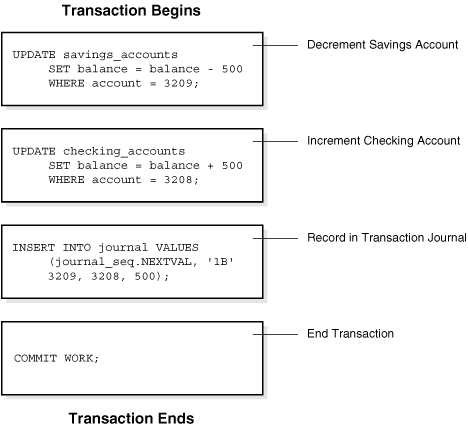
\includegraphics[scale=0.5]{obrazky/sql_transakce}
\par\end{centering}
\caption{Databázová transakce \cite{oracle_transactions} \label{fig:oracleTransactions}}
\end{figure}

\pagebreak
\section{Možnosti replikace a škálovatelnosti}
Při návrhu většiny dnes používaných SQL databázových serverů nebyla brána v úvahu dobrá podpora škálovatelnosti,  možnosti běhu v tzv. \emph{distribuovaném prostředí} tedy na několika serverech zároveň. V dobách jejich vývoje byl totiž Internet značně odlišný o toho jaký známe dnes, neexistovali tak obrovská datová úložiště s nutností rychlého a paralelního přístupu. V dnešní době všechny majoritní SQL servery podporují replikaci a společně s load balancerem \footnote{Server, který shromažďuje požadavky na databázi a rozděluje je rovnoměrně mezi všechny připojené databázové servery.} lze také dosáhnout velmi vysokého výkonu. Sofistikovaným řešením je například technologie MySQL Galera Cluster, která umožňuje provozovat plnohodnotný databázový cluster i s klasickou relační databází MySQL. Data mezi jednotlivými servery jsou transakčně replikovány, zátěž rozděluje vestavěný load balancer. Tato technologie také částečně umožňuje horizontální škálování přidáním serverů, podobné tomu, kterým disponují nové NoSQL databáze  \cite{galeracluster}.

\chapter{NoSQL databáze}
Pojem NoSQL, poprvé použitý Carlem Strozzim v roce 1998 \cite{strozziNoSQL}, je obecný pojem zastřešující všechny databáze nepostavené na tradičním principu relačních SQL databází popsaného v předchozí kapitole. Zahrnuje tedy velké množství databázových serverů a technologií, které  vycházejí ze společné myšlenky.
Především je důležité zdůraznit, co NoSQL není – rozhodně to není NO SQL, tedy trendy odmítání relačních databází. Zkratka NoSQL znamená Not Only SQL, tedy uvědomění si toho, že relační databáze není jediná možnost řešení persistence dat. Že existují také alternativy, které mohou být v některých případech vhodnější. Zrod mnoha NoSQL databází je spjat s projekty známých internetových firem, které se musely vypořádat s obrovským množstvím dat – Facebook (Cassandra), Google (BigTable), Amazon (Dynamo), LinkedIn (Voldemort) atd. \cite{augiNoSQL}
O další rozdělení NoSQL databází se pokusilo už mnoho autorů, jako základní obecné kritérium pro další rozdělení je brán model ukládání dat.  Dále rozlišujeme tedy podle Ricka Cattella \cite{cattellStores} takto.

\begin{table}[h]
\centering
	\caption{Rozdělení NoSQL databázových serverů podle typu úložiště \cite{cattellStores}}
	\begin{tabular}{ |p{5cm}|p{5cm}| }
	\hline
	Typ NoSQL databáze & Databázové servery \\ \hline
	Key-Value Stores & Redis, Scalaris, Tokyo Tyrant, Voldemort, Riak, Memcached \\ \hline
	Document Stores & SimpleDB, CouchDB, \\
	& MongoDB, Terrastore \\ \hline
	Extensible Record Stores & BigTable, HBase, HyperTable, Cassandra \\ \hline
	Graph databases & Neo4j, FlockDB, \\ & AllegroGraph, GraphDB, \\ & InfiniteGraph \\ \hline
	Search Engines & ElasticSearch, Solr,\\ & Sphinx, Splunk \\ \hline
	\end{tabular}

	\label{tab:rozdeleniNoSQLServeru}
\end{table}
NoSQL databáze nebyly navrženy jako náhrada klasických SQL serverů, ale spíš si kladly za cíl vyřešit problémy, na něž současné SQL relační řešení nestačily. Některé typy webových aplikací totiž nevyžadují složité mechanismy ochrany dat, velké množství datových typů nebo transakční zpracování. Naopak vyžadují velmi rychlou odezvu a dostupnost. Proto první implementace NoSQL databází uměly pouze uložit nějakou hodnotu pod unikátním klíčem, sám databázový server nerozuměl hodnotám, které má uloženy a jen je "tupě"  vracel. Tyto NoSQL servery se používají i v dnešní době k ukládání velkých objemů jednoduchých dat (viz. \ref{section:keyValueDB}). Postupem času vzniklo několik skupin databázových serverů s rozdílnými vlastnostmi a způsobem uložení dat. Byly vytvořeny NoSQL databáze, podporující transakční zpracování. Vznikly také velmi zajímavé grafové databáze, které reprezentují relace mezi entitami pomocí hran grafu. Tyto databáze byly ale velmi koncepčně odlišné od klasických SQL databází, hlavně proto,že byly úzce přizpůsobeny pro řešení určitého problému a ani nebyly navrženy jako jejich náhrada. Řešením, které bylo navrženo jako alternativa k SQL serverům, byly \emph{dokumentově orientované NoSQL databáze} (viz. \ref{section:documentsDB}).
V těchto databázích se na entity pohlíží jako na dokumenty, které je možno shlukovat do pojmenovatelných množin (kolekcí) a pracovat s nimi velmi podobně jako s tabulkami SQL serveru.
Nejznámějším zástupcem dokumentově orientovaných databází je MongoDB, tutu databázi lze ve webové aplikaci použít ke stejnému účelu jako například MySQL.
\section{Výhody NoSQL databází}
Hlavní výhodou principu NoSQL databází je hlavně jejích jednoduchost a s tím spojená rychlost. Tato výhoda je ale zároveň i částečnou nevýhodou, jelikož se možnosti dotazování velmi omezily, je třeba složitější operace s daty provádět na straně aplikačního serveru vykonávacího obsluhu databáze. 
Mezi další výhody patři velmi dobrá podpora horizontálního škálování, tedy běhu na více serverech zároveň. S tím spojená schopnost práce s velmi velkými objemy dat, schopnost jednoduché replikace a flexibilní datové modely (neexistují schémata pro strukturu vstupních dat). Často jsou z těchto důvodů nasazovány na tzv. BigData aplikace, tedy aplikace, které pracují s velmi velkou množinou dat a potřebují s nimi rychle a efektivně pracovat. V posledních několika letech se objevilo velké množství nových databázových serverů, které pokrývají celou řadu oblastí při vývoji informačního systému. Můžeme dokonce NoSQL databáze používat jako primární úložiště dat, úložiště MongoDB nabízí vlastní souborový systém GridFS, který ukládá binární data po částech na více databázových serverech, čímž je činní velmi rychle dostupná. \cite{mongoDocs}

\subsection{Schemaless design}
Jedním z největších rozdílů mezi NoSQL a SQL databázemi je fakt, že vkládaná data nemají žádné předem dané schéma, jak mají vypadat. Tento fakt umožňuje vývojářům flexibilněji pracovat s datovými modely. Entita uložená v NoSQL databázi může nabývat mnoha podob, většinou se jedná o nějakou formu objektu, reprezentujícího objekty reálného světa s libovolným množstvím dvojic klíč - hodnota. NoSQL databáze je tedy úložištěm XML, YAML, JSON nebo BSON objektů. Těmto objektům se často říká záznamy nebo dokumenty. Hodnotou takového dokumentu může být i pole, další objekt nebo dokonce pole objektů. Schopnost téměř nekonečného zanořování objektů je další velkou výhodou datového modelu NoSQL databází.

Existuje několik tzv. objektových notací, jenž popisují přechod od objektu k řetězci. Tento proces se nazývá \emph{serializace dat}. Často používanou notací v NoSQL databázích je JSON, tuto notaci používá i NoSQL databáze MongoDB, který je použita v této práci. Vnitřně ovšem MongoDB ukládá tzv. BSON dokumenty, což je ale pouze binární obdoba formátu JSON.
\begin{figure}[h]
\begin{centering}
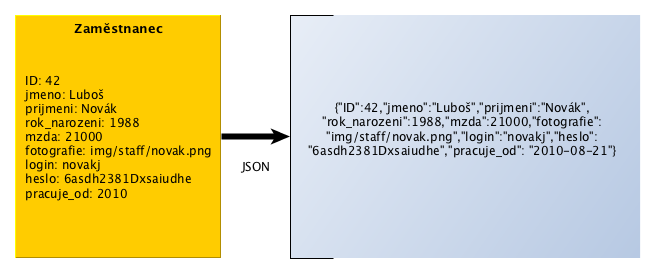
\includegraphics[scale=0.5]{obrazky/json-diagram} 
\caption{Ukázka konverze objektů notací JSON}
\end{centering}
\end{figure}

Pokud je potřeba v NoSQL databázích realizovat relaci mezi objekty, používají se identifikátory již existujících objektů jako prosté řetězcové hodnoty. Tento princip je velmi podobný mechanismu cizích klíčů ze světa SQL databází, NoSQL servery však tento mechanismem nedisponují. Databázový server tuto relaci nevidí a nemůže tedy kontrolovat její splnění, stejně tak získání obsahu odkazovaného objektu je nutné provést až v aplikaci.

\subsection{Sharding, distribuovaný návrh}
V době každý den narůstajících objemů dat, na Internetu uložených, je nutné s těmito daty rychle a účinně pracovat. Proto byly NoSQL databáze navrženy s ohledem na předpokládaný běh na více serverech. Díky tomu, že databáze běží ve více instancích, lze dobře rozdělovat zátěž, generovanou aplikací a jejími klienty. V současné době vzniká u některých aplikací také potřeba dynamicky upravovat výkon, vzhledem k vytížení aplikace jejími uživateli. Náhlé skokové nárůsty zátěže mohou nastat, ale díky distribuovanému návrhu většiny NoSQL databází, lze na tyto nárůsty dobře a rychle reagovat. Tato vlastnost moderních NoSQL databází se nazývá horizontální škálovatelnost a znamená zvýšení výkonu systému přidáním dalších serverů, nikoli zvýšením výkonu stávajících serverů (vertikální škálování). Dobrým příkladem jsou sportovní akce, které prakticky vždy zvýší požadavky na spojení s některými, často televizními, aplikacemi. Výkon databázového clusteru lze řidit i automaticky, existují nástroje, které v případě vysoké zátěže clusteru, automaticky vytvoří další virtuální servery.

Databáze MongoDB je od samého počátku jejího vývoje připravena k provozu v distribuovaném prostředí. K tomu tato databáze nabízí zajímavou funkcionalitu, tzv. \emph{sharding}. Jedná se o způsob rozdělení dat mezi servery zapojené v clusteru. Slovo shard, jak je v tomto případě nazýván jeden databázový server, lze do češtiny přeložit jako střep. Toto dělení obsahu databáze zmenšuje velikost dat, které musejí být uloženy na jednom serveru. Velikost uložených dat značně ovlivňuje rychlost zpracování požadavku nebo rychlost indexování databáze. Každý z těchto serverů obsahuje svojí část dat, která dohromady tvoří celou databázi. Je také možné definovat vlastní kritéria tohoto rozdělování, lze tedy například nová data ukládat na bližším serveru a ty starší mít uloženy jinde. Komunikaci v MongoDB clusteru řídí hlavní server, který také zajišťuje obsluhu požadavků na databázi \cite{mongoCluster}.

NoSQL databáze Redis není určena pro ukládání velkých objemů dat, a proto také neumožňuje ukládat svá data odděleně po částech mezi servery v clusteru. I přes to je Redis také často provozován v clusteru, jednotlivé servery tu zprostředkovávají čtení dat pro klienty, ukládání řídí hlavní databázový server. Redis cluster tedy využívá tzv. \emph{master-slave} architekturu  \cite{panykoNosql}.
\subsection{MapReduce a další agregační funkce}

Jednou z důležitých vlasností relačních SQL databází jsou agregace (shrnutí) dat. Jedná se o způsoby seskupování dat do celků podle zadaných kritérií. Většina NoSQL databází také disponuje bohatými agregačními možnostmi, plně podporující často používané způsoby agregace dat. Neznámější agregační funkcí je \emph{count}. Jejím úkolem je spočítat počet záznamů v databázi, které odpovídají dotazu. Dalšími často používanými agregačními funkcemi jsou funkce \emph{max} a \emph{min}, které slouží z zjištění maxima respektive minima. Lze také použít funkci \emph{group} pro prosté seskupení hodnot, podobné SQL příkazu \emph{GROUP BY}. Nebo je možné využít speciální agregační funkci zvanou \emph{MapReduce}. Tato funkce umožňuje programovat specializované agregace dat, většinou napsané v Javascriptu. Je tak možné získávat nová data nebo fakty ze stávající množiny dat. NoSQL databázové clustery dokonce tuto operaci distribuují mezi jednotlivé servery a zvyšují tím její výkon. Fungování tohoto principu popisuje následující schéma.

\begin{figure}[h]
\begin{centering}
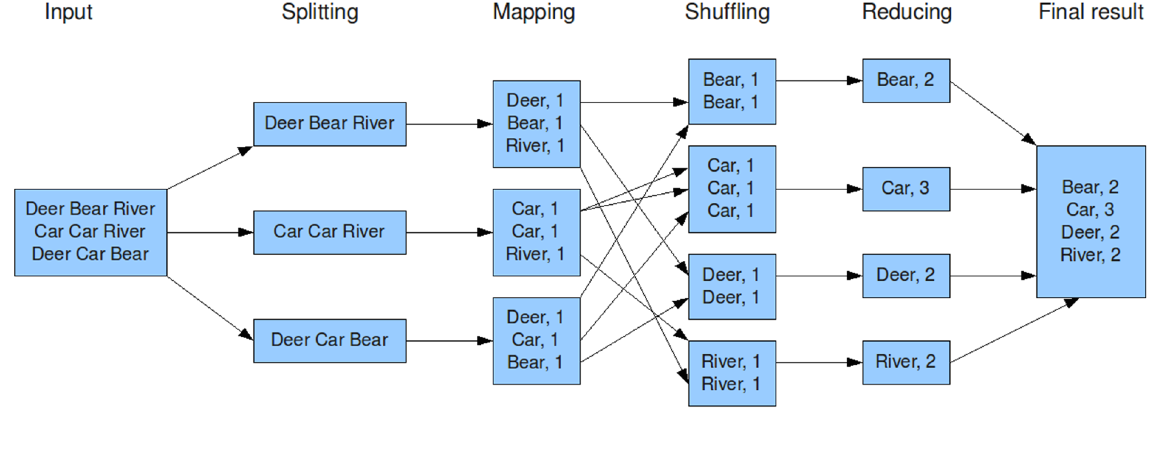
\includegraphics[scale=0.3]{obrazky/mapreduce}
\par\end{centering}
\caption{Ilustrace algoritmu MapReduce \cite{nosqlIrena}}
\end{figure} 
\FloatBarrier
\subsection{Master-Slave Replikace}
Většina z dnes používaných NoSQL databází nabízí nějakou formu zálohování dat. K výpadkům a haváriím vždy dochází a vysoká dostupnost jsou spolu s ochranou dat stěžejními předpoklady moderních NoSQL databází. Nejčastějším řešením tohoto problému je využití dvojic serverů, kde jeden slouží jako hlavní a druhý jako záložní. Úkolem hlavního serveru je zpracovávat požadavky na data a řídit samotnou databázi (mazání expirovaných dokumentů a další obslužné rutiny). Záložní server pouze drží kopii dat hlavního serveru, který se stará o její obnovování. Tento proces se nazývá \emph{master - slave replikace}, jednotlivé dvojice serverů potom většinou \emph{replica sety}. Tyto replica sety jsou popsány v praktické části, jsou totiž základní stavební jednotkou MongoDB databázového clusteru. 

Mechanismy zotavení databáze při výpadku hlavního serveru se mezi NoSQL databázemi značně liší. Dokumentově orientovaná databáze MongoDB používá mechanismus automatického přepnutí rolí serverů, tedy v případě pádu hlavního serveru převezme jeho úlohu server záložní, který se v tu chvíli stává hlavním. Připojíme-li ale původně hlavní databázový server zpět, stane se sám záložním serverem \cite{peteraMongo}. Podobný mechanismus používá i NoSQL databáze Redis, ta však například umožňuje připojit k slave serveru ještě další slave servery, pro které potom původní slave server vystupuje jako master. Problémem vícenásobné replikace je fakt, že operace zápisu je nutné vždy provádět na nejvýše postaveném serveru. Ostatní servery mohou uspokojovat požadavky klientů na data \cite{panykoNosql}. Tyto databáze se nazývají tzv. eventuálně konzistentní (Redis, MongoDB apod.), protože slave servery určené jen pro čtení se vždy nenachází v konzistentním stavu.

\begin{figure}[h]
\begin{centering}
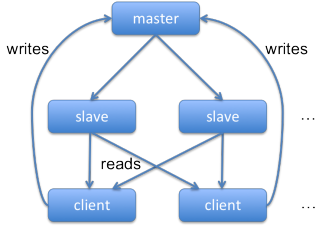
\includegraphics[scale=1.5]{obrazky/master-slave}
\par\end{centering}
\caption{Ukázka eventuální konzistence a komunikace mezi Master a Slave servery v MongoDB \cite{mongoConsist}}
\end{figure}
\pagebreak
\section{CAP teorém}
V roce 2000 na konferenci PODC představil Eric Brewer tři požadavky na distribuovaný systém, které údajně nemůžou být současně splněny. Definoval tři vlastnosti webové aplikace, které jsou bezpochyby žádoucí a od moderní aplikace očekávatelné, ale cíle těchto požadavků se navzájem vylučují \cite{gilbertCap}. Pro tento problém se vžil název \emph{Cap teorém}.

Tento teorém se skládá ze tři částí: Consistency (Konzistence), Availibility (Dostupnost) a Partition tolerance (Tolerance k rozdělení) \cite{cap}.

\vspace{0.25cm}
\noindent Gilbert a Lynch jako první definovali tyto části takto: \cite{gilbertCap}
\begin{itemize}
\item Konzistence (Atomická data) - V každém okamžiku jsou na všech uzlech distribuovaného systému stejná data
\item Dostupnost - Každý připojený klient bude obsloužen, i když chybovou hláškou.
\item Partition tolerance - Tento pojem znamená odolnost vůči výpadkům části distribuovaného systému.
\end{itemize}
Brewer ve své práci uvedl že všechny tři požadavky CAP teorému nelze nikdy splnit na 100\%  \cite{cap}. Z ilustrace teorému \ref{fig:cap} je dobře patrné, že nelze navrhnout databázový systém, který by zcela uspokojil všechny tři jeho požadavky. Další věcí, která je na schématu patrná, jsou tři skupiny databází, splňující alespoň dva požadavky teorému. Zástupce skupiny AP (\emph{Dostupnost a tolerance k rozdělení}) NoSQL databáze Dynamo klade důraz na to, aby každý připojený klient dostal odpověď na svůj dotaz a to i v případě výpadku napájení. U databáze HBase, patřící do skupiny CP (\emph{Konzistence dat a tolerance k rozdělení}), je zase hlavní konzistence dat \cite{panykoNosql}. Tradiční relační databázové systémy se označují jako CA (Konzistence a Dostupnost). 

Moderní NoSQL řešení se většinou vzdávají silné konzistence, aby získaly vyšší dostupnost. Tyto databáze pak nazýváme jako \emph{eventuálně konzistentní} \cite{peteraMongo}. Do této skupiny patří i databáze MongoDB, kterou se hlouběji zabývá tato práce \cite{mongoConsist}.

\vspace{0.5cm}
\noindent\emph{Jednotlivé skupiny databázových systémů, které splňují alespoň dvě části teorému.}
\begin{itemize}
\item AP (Availibility + Partitioning) - Dynamo, Voldemort, Cassandra
\item CP (Consistency + Partitioning) - MongoDB, Redis, HBase
\item CA (Consistency + Availibility) - MySQL, MSSQL, 
\end{itemize}

\begin{figure}[h]
\begin{centering}
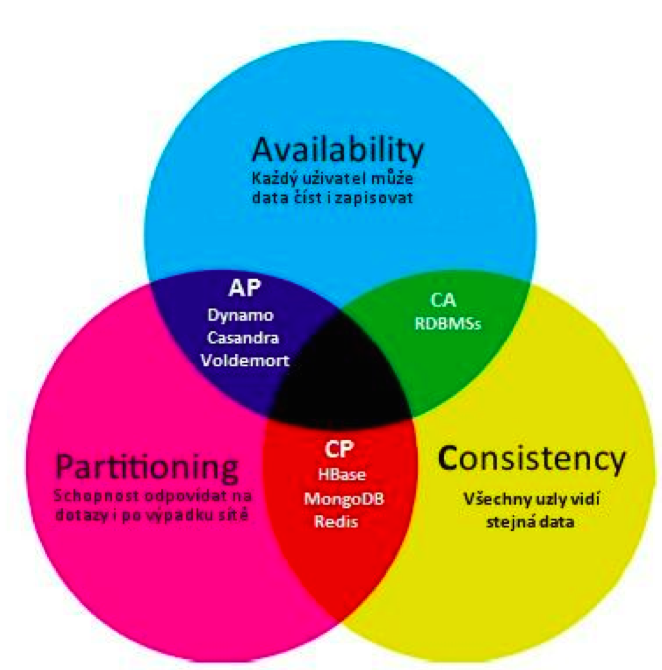
\includegraphics[scale=0.3]{obrazky/cap}
\par\end{centering}
\caption{Ilustrace CAP teorému \cite{panykoNosql}\label{fig:cap}}
\end{figure}

\section{BASE}
BASE byl navrhnut jako standard pro moderní ukládání velkých objemů dat v distribuovaných systémech. Je přímou reakcí na standard ACID u relačních databází. Tento princip za cenu omezení konzistence dat, zvyšuje jejich dostupnost. Christof Strach ho popisuje takto:\cite{strauchNosql}
\begin{itemize}
\item Basically Available - Systém stále běží, mohou nastat jen částečné chyby, nezpůsobující pád systému
\item Soft State - Systém je pružný, změny mohou nastávat (a nastávají) neustále
\item Eventual Consistency - Očekávání konzistentního stavu v budoucnu
\end{itemize}

\vspace{0.25cm}
\FloatBarrier
\begin{table}[h]
\caption{Srovnání ACID vs. Base \cite{nosqlSlides}}
\noindent\begin{tabular}{p{6.5cm} p{6.5cm}}
ACID (SQL) & BASE (NoSQL)\\ \hline
silná konzistence & slabá konzistence (stará data) \\
izolovanost & dostupnost na prvním místě \\
orientace na commit & přibližné odpovědi jsou OK \\
vnořené transakce & jednodušší, rychlejší \\
nezaručená dostupnost & dodávka dat "jak to jen půjde" \\
konzervativní (pesimistické) & agresivní (optimistické) \\
složitá evoluce kvůli schématu & jednoduchá evoluce (schemaless) \\
\end{tabular}

\end{table}
Případné nekonzistence jsou řešeny při čtení (verzování nebo nevalidní cache), při zápisu (distribuce změn) nebo asynchronně při replikaci dat \cite{nosqlSlides}.
\section{Typy NoSQL databází}
NoSQL databázový server je typicky jednoduché úložiště typu klíč -> hodnota, kdy hodnotou může být cokoliv (nejčastěji strukturovaný objektový zápis např. JSON) a klíč bývá unikátní identifikátor vygenerovaný samotnou databází. Toto je jedna z největších výhod těchto řešení, neomezuje totiž programátory žádnými modely předepisujícími strukturu vkládané entity. Typickým zástupcem takto jednoduché databáze je například Redis. 

Rozšiřujícím prvkem nad těmito úložišti může být další logické rozdělení uložených hodnot. Toto poskytují například dokumentově orientované databáze (např. MongoDB), kde každá vložená entita je uložena do nějaké kolekce, popisující typ a zařazení této entity. Díky návrhu podobnému SQL (kolekce vs. tabulky), jsou dokumentově orientované databáze použitelné jako přímá náhrada relačního SQL řešení.

Kvůli potřebám velmi rychlé správy propojených dat, vznikly také grafové databáze, které ukládájí dat a jejich vazby pomocí grafových struktur.

\subsection{Key-value úložiště}
\label{section:keyValueDB}
Prvním a také nejstarším typem NoSQL databází jsou key-value úložiště. Impulsem pro jejich vznik byla potřeba velmi rychle ukládat jednoduchá data s krátkou dobou uchování, často jen unikátní řetězce sloužící k nějaké formě identifikace.
Key-value databáze obecně je úložiště, kde každá uložená entita je indexována jen a pouze svým klíčem, nejčastěji nějakým unikátním identifikátorem ve formě řetězce. 
Vnitrně bývá implementováno jako jednoduchá hash tabulka \footnote{Datové struktura, sloužící k ukládání dvojic klíč-hodnota. Hashovací tabulka kombinuje výhody vyhledávání pomocí indexu a procházení seznamu.} nebo mapa \cite{beltrameKeyValue}.  

\vspace{0.5cm}
\noindent Tyto úložiště většinou poskytují jen tři nejzákladnější operace ke svojí obsluze a to:
\begin{itemize}
\item Uložení entity pod nějakým klíčem, ten je buď definován ve vstupních datech nebo vygenerován databázovým serverem
\item Získání entity podle klíče
\item Smazání entity podle klíče
\end{itemize}
Typů entit existuje velké množství, které je závislé na dané implementaci databáze. Key-value databáze Redis například nabízí řetězce, seznamy, mapy nebo množiny. Do těchto datových typů lze ukládat jednoduché řetězce i složité objekty \cite{redisDocs}.
Tato jednoduchost návrhu přináší velmi vysokou rychlost zpracování dat a jednoduchou škálovatelnost, je ale nutné veškeré složitější operace s daty provádět na aplikačním serveru. Databáze tedy skutečně zůstává jen tenkou vrstvou k uložení dat, která jsou však velmi rychle dostupná, díky možnosti běhu databáze na různém počtu strojů podle aktuální potřeby. Většina implementací key-value databází si drží svá data přímo v paměti, tato data jsou díky tomu ještě rychleji dostupná.
Důležitou vlastností key-value databází je možnost nastavení doby expirace uložených záznamů. Po uplynutí této doby se záznam v databázi automaticky smaže. Tato vlastnost je často využívána při ukládání uživatelských sezení, kdy expirace záznamu v databázi znamená odhlášení uživatele z aplikace z důvodu dlouhodobější nečinnosti \cite{redisDocs}.

Někteří zástupci těchto databází v omezené míře podporují transakční zpracování. Redis umožňuje řadit příkazy do fronty a pak je provést všechny najednou. V tomto případě databáze garantuje že příkazy uvnitř fronty budou provedeny najednou a žádný jiný požadavek nemůže být vyřízen, dokud se celá transakce nedokončí. Příkazy v transakci se provedou buď všechny úspěšně nebo dojde k jejímu selhání. Zde můžeme nalézt analogii se světem SQL databází, ale na rozdíl o SQL serverů, Redis nepodporuje žádný mechanismus, který by se dal přirovnat k příkazu \emph{ROLLBACK}, známým z SQL transakcí. Databáze tedy neposkytuje žádnou možnost reagovat na selhání transakce. Redis také disponuje možností master-slave replikace, která probíhá asynchronně, což umožňuje pracovat s databází i v průběhu replikace. Pro zajištění velmi vysoké dostupnosti databáze, je vyvíjen nástroj Redis Sentinel, umožňující automatickou správu Redis clusteru. Tento nástroj umožňuje monitorování běžících instancí Redisu, jejich obsluhu a automaticky přepíná mezi dvojicemi replikovaných serverů, pokud dojde k výpadku některého z nich \cite{redisDocs}.

Tyto databáze zajišťují ukládání dat pro specifickou oblast webové aplikace, pro kterou jsou výborně optimalizovány, například slouží jako úložiště uživatelských sezení nebo kešovaných dat. Kvůli jejich úzké specializaci není ve většině případů absence plnohodnotných transakcí problém. 
Mezi nejznámější key-value úložiště patří vedle již zmíněného Redisu, také Riak, Dymamo, Voldemort, Berkeley DB, HamsterDB nebo Memcached. 
Do této kategorie patří také Cassandra, jedna z prvních NoSQL databází vyvinutá ve společnosti Facebook \cite{cassandra}.

Většina key-value databází včetně Redisu je volně dostupná. Redis je dokonce distribuován pod licencí BSD, je ho tedy možná zdarma používat i na komerčních projektech \cite{redisDocs}.

\begin{figure}[h]
\begin{centering}
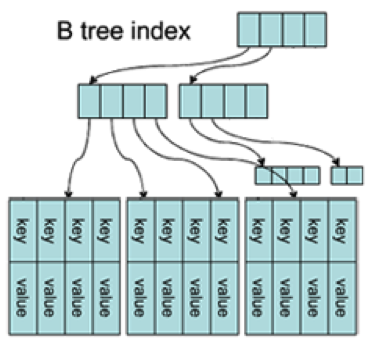
\includegraphics[scale=1]{obrazky/keyvaluedb-strom}
\par\end{centering}
\caption{Ukázka uložení dat v key-value databázích \cite{tolitStorelist} \label{fig:keyValueTree}}
\end{figure}

\subsection{Dokumentově orientované databáze}
\label{section:documentsDB}
Dokumentově orientované databáze představují evoluci NoSQL databází, nabízejí kompromis mezi přílišnou jednoduchostí a dostatečnou rychlostí zpracování. Jejich  nejznámější zástupce, MongoDB, je dlouhodobě nejpoužívanější NoSQL databázi nasazovanou do ostrého provozu  \cite{enginesRanking}.
MongoDB je také jednou ze dvou databází, kterou se hlouběji zabývá tato práce. Tato databáze byla vyvinuta společnost 10gen v roce 2007, jako součást své platform-as-a-service platformy. V roce 2009 tato společnost vydala první open source verzi své databáze. Název této NoSQL databáze je odvozen od anglického slova "humongous", které popisuje něco velmi velkého nebo chcete-li obrovského.  Stabilní verze, připravená pro produkční nasazení, vyšla v roce 2010. MongoDB je napsáno v jazyce C++. Tato databáze byla od začátku navržena pro běh v clusteru, jedná se proto o jednu z jejich klíčových vlastností  \cite{peteraMongo}.

Základním prvkem pro ukládání dat je zde dokument, kterým je míněn objekt (entita) s jedinečným identifikátorem a množinou párů klíč-hodnota, jež mohou být do sebe dále libovolně vnořovány. Na rozdíl od systémů typu klíč-hodnota většinou umožňují také sekundární indexování atributů \footnote{Možnost přidání indexu na kterýkoliv klíč entity.},  a co do funkcionality jsou robustnější. Pro ukládání dat užívají JSON, XML nebo podobné strukturované formáty  \cite{regnerVse}.
Dalším důležitým prvkem je kolekce, která popisuje a obaluje dokumenty, v ní uložené. Vnitřní rozdělení dokumentů do kolekcí doplňuje logické uspořádání entit do celků, podle nichž lze dokumenty opět získávat. Pro získání všech dokumentů určitého typu, už tedy není potřeba žádná složitější aplikační logika, stačí jen získat celou kolekci.

Kolekce v MognoDB fyzicky obsahuje libovolný počet BSON \footnote{Binární podoba formátu JSON.} dokumentů, jehož maximální možná velikost je 16MB. Větší dokumenty lze ukládat pomocí souborového systému GridFS, který rozdělí dokument a několik částí (chunků) a ty poté obsluhuje jako jeden dokument. Dotazovacím jazykem databáze MongoDB je Javascript. V tomto jazyce lze také psát vlastní uložené procedury \cite{mongoDocs}. 

Kvůli tomu je tato databáze velmi oblíbená především u vývojářů moderních javascriptových SPA\footnote{Single Page Application - jednostránková webová aplikace, napsaná kompletně v klientském Javascriptu.} a mezi vývojáři v NodeJS. Databáze MongoDB je distrubována pod licencí GNU AGPL v3.0 pro serverovou část a Apache 2 Licence pro klientskou část, je tedy možné ji používat zdarma i pro komerční využití.

\begin{lstlisting}[caption=Příklad databázového dotazu v MongoDB]
db.zamestnanci.find(
    {
       prijmeni: 'Novak',
       mzda: {'$gte':10000}
    }
);
\end{lstlisting}
\noindent Tento dotaz vyhledá v kolekci \emph{zamestnanci} všechny zaměstnance kteří je jmenují Novák a mají mzdu větší než 10000 Kč.
Funkce \emph{find()} slouží k získávání dat z kolekce pomocí definovaných omezení. Je ekvivalentem příkazu SELECT u SQL databází. První parametrem funkce je tzv. \emph{matcher}, který udává podmínky, jenž musí splňovat entita v kolekci. V našem případě musí obsahovat příjmení Novák. Konstrukce \$gte je z anglického "\emph{greater than equals}" a znamená matematickou operaci větší nebo rovno. Funkce \emph{find()} umožňuje používat i druhý parametr, tzv. projekci. Ta umožňuje definovat strukturu vrácených dokumentů, projekce tedy funguje naprosto stejně jako výčet sloupců v SQL příkazu SELECT \cite{mongoDocs}.
\pagebreak

\begin{lstlisting}[caption=Odpověď MongoDB databázového serveru]
{
   jmeno: 'Pavel',
   pozice: 'Manager',
   prijmeni: 'Novák'
   mzda: 15800,
   oceneni: [
   	{nazev: 'Nejlepší Manažer 2014', udeleno: 2014-07-08}
   	],
   umisteni: 'management',
   fotografie: 'images/staff/pnovak.png',
   prava: ['user','manager'],
   ve_spolecnosti: 2001
}

{
   jmeno: 'Jiří'
   prijmeni: 'Novák',
   pozice: 'Accountant',
   umisteni: 'ekonomicke',
   mzda: 11200,
   ve_spolecnosti: 2010
}
{
   jmeno: 'Jakub'
   prijmeni: 'Novák',
   pozice: 'Developer',
   umisteni: 'developers',
   mzda: 37000,
   prava: ['user','developer'],
   ve_spolecnosti: 2005
}
\end{lstlisting}

Kolekci není potřeba nijak vytvářet, je vytvořena automaticky při vložení prvního záznamu. Přepínání mezi databázemi probíhá analogicky s SQL světem pomocí příkazu \emph{USE}. Data se vkládají pomocí příkazu \emph{insert}, jejímž jediným parametrem je dokument ve formátu JSON, který bude uložen do zvolené kolekce. Kolekce, nad níž provádíme operace, se v MongoDB uvádí jako objekt, nad kterým voláme funkce \emph{find} nebo \emph{insert} \cite{mongoDocs}.

\pagebreak
\begin{lstlisting}[caption=Vložení dokumentu do databáze test a kolekce zamestnanci v MongoDB]
use test;
db.zamestnanci.insert(
	{
		jmeno: 'Jakub',
		prijmeni: 'Josef',
		pozice : 'CEO',
		umisteni: 'management',
		mzda: 250000,
		fotografie: 'images/hq/jjosef.png',
		prava: ['user', 'manager', 'hq', 'admin'],
		ve_spolecnosti: 2000 	
	}
);
\end{lstlisting}

Unikátní identifikátor záznamu (v SQL světě známý jako primární klíč) v MongoDB nalezneme pod klíčem \emph{\_id}. Pokud není \_id specifikováno ve vkládaném dokumentu (jako v ukázce výše), bude automaticky vytvořeno databází. Databáze MongoDB generuje 12 bytový řetězec, který se skládá z náhodného čísla, data vytvoření dokumentu a jedinečného identifikátoru stroje a procesu  \cite{mongoDocs}.

Kolekce v MongoDB lze také omezit maximálním počtem záznamů (tzv. Capped Collections), tyto kolekce se výborně hodí pro ukládání dat, které je třeba uchovávat pouze po omezenou dobu, například nějaké souhrny nebo logy. Ukládání dat do kolekce lze omezit také časově. Samotné dokumenty v MongoDB také umožňují expiraci (odstranění) dokumentu po určitém čase. Tomuto parametru se říká TTL\footnote{Time to live.} a v MongoDB se nastavuje jako index \cite{mongoDocs}.

\begin{lstlisting}[caption=Vytvoření indexu s parametrem expirace TTL 3600 sekund]
db.log_events.ensureIndex( { "createdAt": 1 }, { expireAfterSeconds: 3600 } )
\end{lstlisting}

Pro pokročilejší získávání dat lze v MongoDB používat i tzv. matchery, kterými lze definovat kritéria, podle nichž lze výběr omezit. Matchery vždy začínají znakem \$ a nabízejí bohaté možnosti dotazování, řeší chybějící operátory v dotazech a jsou přímým NoSQL ekvivalentem příkazu WHERE ze světa SQL databází. Samotný MongoDB matcher je klasický objekt, na jehož klíči je název matcheru (operátor) a hodnotou je hodnota, která bude argumentem operátoru. Jednotlivé matchery lze shlukovat pomocí logických operátorů \emph{\$and},  \emph{\$or} a \emph{\$not} \cite{mongoDocs}.
\pagebreak

\noindent\emph{Nejčastěji používané matchery v MongoDB}
\begin{itemize}
\item \$gt - hodnota prvku je větší než, ekvivalent znaku >
\item \$gte - hodnota prvku je větší nebo rovno, ekvivalent znaku >=
\item \$lt - hodnota prvku je menší než, ekvivalent znaku <
\item \$lte - hodnota prvku je menší nebo rovno, ekvivalent znaku <=
\item \$ne - hodnota prvku je se nerovná, ekvivalent znaku !=
\item \$nin - prvek neexistuje
\item \$exists - existuje klíč
\item \$type - klíč je specifického typu
\item \$mod - operace modulo, ekvivalent znaku %
\item \$regex - dotazování pomocí regulárního výrazu
\item \$text - provede fulltextové vyhledávání
\item \$where - hodnota prvku bude porovnána pomocí Javascriptové funkce
\item \$all - hodnotou prvku je pole a obsahuje všechny zadané prvky
\item \$elemMatch - hodnotou prvku je pole a prvním elementem pole je zadaný element.
\end{itemize}

Matcherů v MongoDB existuje celá řada a pokrývají veškeré běžné matematické operace. Existují také matchery poskytující výpočet tzv. Haversinovské vzdálenosti, tedy vzdálenosti mezi dvěma body v prostoru, zadanými pouze GPS souřadnicemi. K tomu slouží geometrické matchery \emph{\$near} a \emph{\$nearSphere} \cite{mongoDocs}.

\begin{lstlisting}[caption=Ukázka složitějšího dotazu na MongoDB databázi]
db.zamestnanci.find(
   {
     umisteni: 'management',
     prava: 'hq',
     $or: [ { mzda: { $gt: 15000, $lte: 100000} }, { ve_spolecnosti: { $lt: 2010 } } ]
   }
)
\end{lstlisting}

Tento dotaz získá všechny zaměstnance, kteří jsou umístění v sekci management a mají buď mzdu větší než 15000 Kč a menší než 100 000 Kč, nebo jsou ve společnosti déle než 4 roky (v roce 2014). Jinak řečeno, jejich rok nástupu je nižší než 2010. Ačkoliv se na klíči \emph{prava} nachází pole, v dotazu je použit jen prostý řetězec. V tomto případě totiž databáze pole otestuje na existenci tohoto řetězce \cite{mongoDocs}.

Další důležitou vlastností každé databáze je možnost řazení, v SQL prováděné pomocí klauzule \emph{ORDER BY}. MongoDB nabízí metodu \emph{sort()}, která přijímá objekt s klíčem podle kterého bude seřazení probíhat a číslem udávajícím směr tohoto řazení. Směr se v MongoDB udává pomocí dvou čísel, \emph{1} znamená vzestupně a je ekvivalentem SQL klauzule \emph{ASC}. Sestupné řazení (DESC) se v MongoDB udává jako \emph{-1}. Omezení velikosti výsledku je v MongoDB dostupné pomocí jasně použitelné funkce \emph{limit()} příjímající počet dokumentů, které budou vráceny. \cite{mongoDocs}. 

\begin{lstlisting}[caption={Ukázka sestupného řazení podle mzdy a omezení v MongoDB}]
db.zamestnanci.find(...).sort({ mzda: -1}).limit(20)
\end{lstlisting}
Možnosti dotazování jsou v dokumentově orientované databázi MongoDB skutečně bohaté a dalo by se  říci, že dokonce převyšují obvyklé možnosti SQL serverů. Databáze je dostupná pro Linux, Windows, Mac OS X a Solaris.

Dalšími zástupci dokumentově orientovaných databází jsou CouchDB,  RavenDB nebo RethinkDB.
CouchDB je databází, která vychází z dokumentově orientovaného projektu Lotus Notes. Její hlavní vývojář Damien Katz na tomto produktu dlouho pracoval u společnosti IBM. Tato databáze se koncepčně velmi podobná MongoDB, avšak nepoužívá kolekce, ale přináší například pohledy na data nebo replikaci na klientská zařízení. Komunikace s ní probíhá, na rozdíl od MongoDB, pomocí vestavěného REST API. Administrační úkony v databázi je tedy nutné provádět například pomocí nástroje cURL \footnote{Nástroj příkazové řádky usnadňující odesílání HTTP požadavků.} \cite{strauchNosql}.
\subsection{Sloupcově orientované databáze}
Sloupcově orientované databázové systémy vycházejí z projektu Google BigTable  \cite{changBigtable}. Jsou opět určeny především vysokozátěžovým systémům a jsou vysoce optimalizovány pro paralelní zpracování dotazů. Můžeme si je představit jako klasickou tabulku. Každý záznam (řádek) zde má svůj unikátní identifikátor, ovšem fyzicky se data ukládají nikoliv po řádcích, jak je běžné u relačních databází, nýbrž po sloupcích. Je tak rychlejší například vyhledat záznamy s určitou hodnotou atributu a zároveň se šetří diskový prostor serveru, jelikož nemusí být vyhrazeno žádné místo navíc pro prázdné buňky \cite{regnerVse}.
Tyto databáze se hodí pro použití v datacentrech, pro CRM systémy\footnote{Customer Relationship Management - Systémy pro řízení vztahů se zákazníky.}, knihovny nebo podobná nasazení. Sloupcově orientované databáze se obecně hodí pro správu velkého množství stejných nebo podobných dat, které ukládají na disk po sloupcích zvlášť. To umožňuje při čtení načíst přesně tolik atributů (sloupců), kolik je zrovna potřeba, a tím šetřit prostředky databázového serveru \cite{columnDB}. 

Následující obrázek \ref{fig:columnDB} dobře ilustruje odlišnosti ve struktuře dat sloupcově orientovaných databází. Pokud aplikace potřebuje nová data a žádá o obsah atributů \emph{saleid} a \emph{date}, databázový server skutečně získá jen tyto sloupce a vrátí jejich obsah. Naopak pokud aplikace často získává celé objekty, nebo provádí agregační funkce, není pro ni sloupcově orientovaná databáze příliš vhodná.

\begin{figure}[h]
\begin{centering}
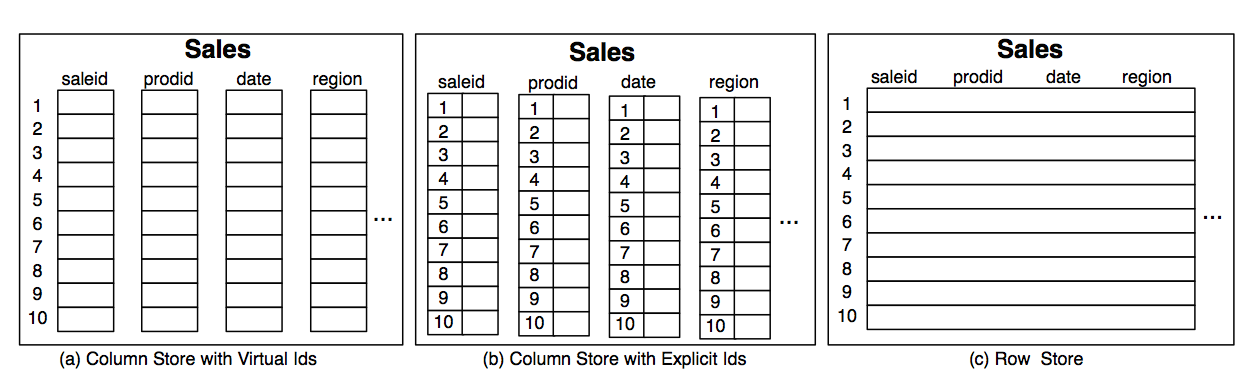
\includegraphics[scale=0.3]{obrazky/column-vs-row}
\par\end{centering}
\caption{Porovnání sloupcově orientované databáze s relační databází založenou na řádcích. \label{fig:columnDB} \cite{columnDB}}
\end{figure}
Mezi nejznámější sloupcově orientované databáze patří MonetDB, HBase, BigTable nebo HyperTable.

\subsection{Grafově orientované databáze}
Grafově orientované databáze představují specifický typ databázových systémů založený na grafech. Tyto databáze se hodí pro reprezentaci sítí a jejich typologii, jako jsou například sítě počítačové, dopravní nebo sociální. Používají se tedy k práci s daty, která mají mezi sebou velké množství vazeb. Do databáze se ukládají uzly s určitými vlastnostmi a také hrany mezi těmito uzly \cite{graphDb}.

Hlavním přínosem je schopnost rychle vyhledávat příslušné uzly i ve velmi rozsáhlém grafu. Grafové databáze totiž při vyhledávaní používají pokročilé grafové algoritmy, které jsou pro dané použití mnohem rychlejší a efektivnější než by byla běžná relační databáze \cite{graphDb}.  

Grafová databáze se obecně skládá ze dvou základních prvků, vrcholů (nodes) a hran (edges). Každý z těchto vrcholů obsahuje několik hran vedoucích k dalším vrcholům. Tyto hrany reprezentují vazby. Hrany mezi vrcholy mají vždy označen směr, víme tedy, ze kterého vrcholu vstupuje a ze kterého vystupuje. Mohou však existovat i vrcholy, které na sobě žádné hrany nemají \cite{graphDb}. 

Samotná data jsou nejčastěji uložena ve vrcholech, ačkoli grafová databáze Neo4j nabízí možnost ukládání dat i v hranách \cite{neo4j}.
Pravděpodobně nejznámější grafovou databází je Neo4j. Tato databáze, která je postavena na programovacím jazyku Java, je velmi oblíbená pro ukládání hustě propojených dat a je k tomuto účelu v poslední době i často nasazována. Na rozdíl o většiny NoSQL databází, databáze Neo4j podporuje ACID transakce. Ty ale drží v paměti, což může být u větších grafů problém. Je proto doporučeno velké transakce dělit na několik menších, pokud nehrozí porušení konzistence dat v databázi. \cite{neo4j}.

Komunikace s Neo4j serverem probíhá přes vestavěné REST API, které nabízí rozhraní dostupné pro vývojáře jakéhokoliv jazyka. Hlavním komunikačním formátem je JSON \cite{neo4j}.

\begin{figure}[h]
\begin{centering}
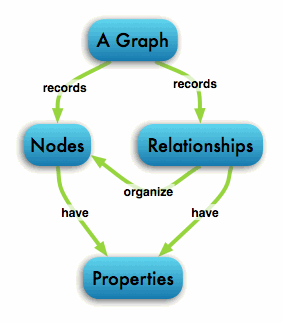
\includegraphics[scale=0.5]{obrazky/neo4j-graph}
\par\end{centering}
\caption{Vztahy mezi entitami v Neo4j. \cite{neo4j}}
\end{figure}

\FloatBarrier
Grafová databáze Neo4j používá speciální dotazovácí jazyk Cypher, pomocí něj je možné vytvářet, získávat, nebo editovat data v databázi. Základem syntaxe tohoto jazyka je vzor, dotazování na data probíhá pomocí mechanismu známého jako \emph{pattern matching} \footnote{Způsob porovnávaní sekvence znaků proti zadanému vzoru.}. Data se tedy získávájí pomocí porovnávání zadaných vzorů a struktury grafu. Samotný vzor se skládá z jednoho nebo více uzlů s jejich vzájemnými vztahy, štítky a vlastnostmi. Vlastnost v Neo4j reprezentuje dvojice klíč - hodnota, která je již v této práci dobře popsána. Druhou důležitou částí jazyka Cypher jsou tzv. klauzule. Klauzule jako takové jsou dobře známým pojmem z SQL databází a jejich syntaxe a použití v Neo4j jsou velmi podobné. Základ jazyka tvojí klauzule \emph{MATCH}, která umožňuje hledání podle zadaného vzoru. Klauzule WHERE slouží k zadání podmínek dotazu, naprosto analogicky jako u SQL databází \cite{cypher}. 
 
\begin{lstlisting}[caption={Ukázka Neo4j dotazu, který získá uživatele s ID 123}]
MATCH (user:User)
WHERE user.Id = 1234
RETURN user
\end{lstlisting}

Modifikace uložených dat funguje podle očekávání prostřednictvím příkazu \emph{SET} \cite{cypher}.
\begin{lstlisting}[caption={Ukázka Neo4j dotazu který provede změnu věku uživatele 123}]
MATCH (user:User)
WHERE user.Id = 123
SET user.Age = 25
\end{lstlisting}

Další klauzule \emph{CREATE, MATCH, SET, REMOVE a DELETE} slouží pro manipulace s daty. V rámci dotazování je také možné používat speciální grafové funkce jako například \emph{shortestPath} pro nalezení nejkratší cesty v grafu, nebo \emph{allPaths} pro nalezení všech přípustných cest \cite{cypher}.
\begin{lstlisting}[caption={Ukázka Neo4j dotazu, který vytvoří nového uživatele,  poté ho spojí s uživatelem 123, který ho pozval (role invitee)}]
MATCH (invitee:User)
WHERE invitee.Id = 123
CREATE invitee-[:INVITED]->(invited:User {newUser})
\end{lstlisting}

Neo4j server je dostupný pro Linux, Mac OS X a Windows ve 4 základních verzích licencovaných podle jejích použití. Základní verze \emph{Neo4j Comunity} je určena pro open source projekty a je distribuována zcela zdarma. Tato verze obsahuje různá omezení, je například ochuzena o monitorovací nástroje nebo clustering. Druhou variantou je verze \emph{Neo4j Personal}, která nabízí plnou verzi databáze zcela zdarma. Tato varianta je ale přípustná pouze pro malé firmy do příjmu 100 tisíc dolarů a maximálně 3 zaměstnanců. Třetí možnost licencování, určená především pro startupy, se jmenuje \emph{Neo4j Startups}. Je k dispozici firmám s ročním příjmem nižším než 5 milionů dolarů a v případě startupů s počáteční investicí nižší než 10 milionů dolarů. Cena této licence je 12 tisíc dolarů (asi 250 tisíc Kč) za kalendářní rok. Ostatním společnostem, které nesplňuji výše uvedená kritéria je cena licence stanovena individuálně \cite{neo4jLicence}.

Další zajímavou grafovou databázi představuje AllegroGraph. Jedná se o zástupce tzv. RDF databází. RDF objekt, v ní uložený, je takzvaný triplet ve tvaru subjekt-predikát-objekt a představuje datový model reality. Můžeme si ho představit jako orientovaný ohodnocený graf, kde hrana začíná v subjektu, je ohodnocena predikátem a končí v objektu. Subjekt představuje datový zdroj, většinou URI. Predikátem se chápe nějaká vlastnost nebo aspekt daného subjektu, vyjadřuje tedy jeho vztah k danému objektu. Tento objekt tvoří hodnotu a může obsahovat čísla nebo řetězce. Častěji je ale objektem URI dalšího subjektu a vznikne tím zřetězení. Tímto způsobem lze velmi dobře popisovat například rodinné vztahy nebo lze nad RDF grafem také dokazovat fakta. Dotazování na RDF databáze většinou realizuje dotazovací jazyk SPARQL \cite{nosqlSlides}.

\subsection{Vyhledávací enginy}
Zvláštní skupinou serverů, které se vlastně také dají považovat za NoSQL databáze, jsou vyhledávací enginy. Tyto databáze jsou vysoce optimalizovány pro rychlé prohledávání velkého množství textových dat. Jejich úkolem je rozložit věty na jednotlivá slova a poté kořeny těchto slov spolu se informacemi o synonymech zaindexovat do vlastní databáze. Zároveň tento engine obsahuje vlastní sadu slov, které se nebudou indexovat, protože se jedná o běžné výrazové prostředky jazyka: jednoduchá slova, předložky nebo spojky. Poté je  možné se fulltextově dotazovat na objekty v ní uložené \cite{searching}.

Z již napsaného vyplývá, že tyto procesy zpracování textových dat je třeba konfigurovat přímo pro daný jazyk ve kterém bude engine používán \cite{searching}. Tyto databáze se využívají především pro účely fulltextového vyhledávání. Proprietární řešení od společností Google nebo Microsoft pravděpodobně používá podobné mechanismy zpracování textových dat.
\begin{figure}[h]
\begin{centering}
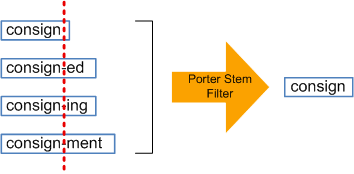
\includegraphics[scale=0.9]{obrazky/stemming}
\par\end{centering}
\caption{Ukázka stemmingu, tvorby kořene slov \cite{grailsLucene}}
\end{figure}

Nejznámějšími zástupci vyhledávacích enginů je Sphinx Search nebo ElasticSearch. Zejména  ElasticSearch se začíná v poslední době často používat pro fulltextové vyhledávání, momentálně je nejpoužívanější databází svého druhu \cite{enginesRanking}.


\section{Monitoring databáze}
Obecně asi každý počítačový server je dobré monitorovat, aby mohl jeho administrátor kontrolovat jeho stav a reagovat na případné problémy. U databázových serverů je důležitost monitoringu vysoká hlavně při použití distribuovaných řešení. Některé z NoSQL databázových serverů již v základu obsahují nějakou formu monitoringu, často tenký webový server zobrazující informace o databázi. Například MongoDB po svém spuštění spouští také webový server obsahující administrační rozhraní. Tento server běží na portu o 1000 vyšším než je nastavený port databáze. Tedy implicitně na portu 28017 \cite{mongoAdmin}. Vestavěné webové  administrační rozhraní obsahuje také grafová databáze Neo4j \cite{neo4jAdmin}. Existuje také velké množství aplikací pro monitoring NoSQL databázových serverů, namátkou lze zmínit například Redsmin pro správu Redis databáze, nebo OpsCenter na monitoring a vizualizaci dat pro databázi Cassandra.

Následující dva obrázky představují ukázku vestavěného webového rozhraní v MongoDB.
Databáze je spuštěna na standartním portu 27017, webové rozhraní je tedy dostupné na portu 28017.
 
\begin{figure}[h]
\begin{centering}
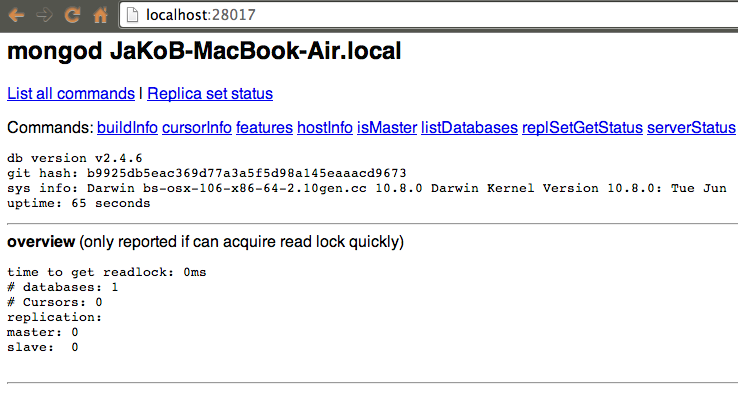
\includegraphics[scale=0.4]{obrazky/mongo-admin-top}
\par\end{centering}
\caption{Stav MongoDB serveru ve webovém rozhraní\label{fig:mongoAdmin}}
\end{figure}

\FloatBarrier
První z nich ilustruje stav serveru, jeho verzi a kód sestavení. Dozvíme se zde také info o systému a dobu běhu serveru. Na druhém obrázku vidíme připojené klienty k databázi. Skutečně připojení klienti vždy začínají slovem \emph{conn}, ostatní jsou systémové rutiny. Například rutina TTLMonitor se stará o mazání expirovaných (neplatných) záznamů \cite{mongoAdmin}.

\begin{figure}[h]
\begin{centering}
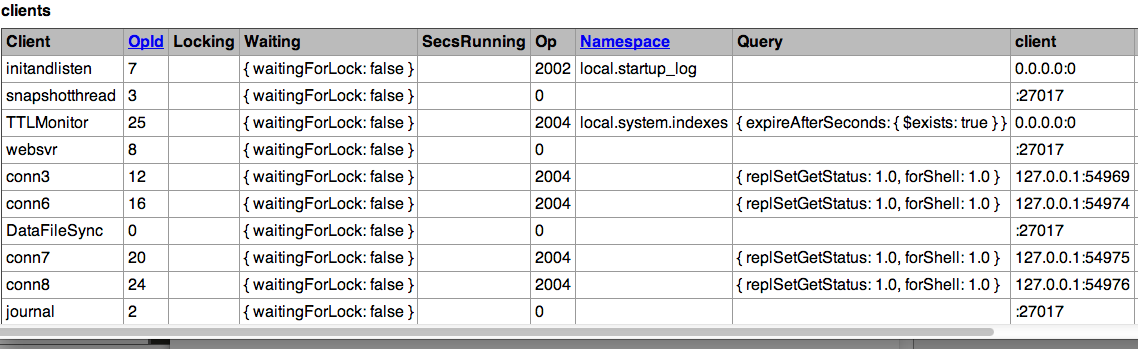
\includegraphics[scale=0.3]{obrazky/mongo-admin-clients}
\par\end{centering}
\caption{Seznam připojených klientů MongoDB serveru ve webového rozhraní\label{fig:mongoAdmin}}
\end{figure}

\FloatBarrier
Grafová databáze Neo4j také disponuje administračním rozhraním, pomocí kterého lze sledovat stav databázového serveru, nebo provádět manipulovce s daty. Toto rozhraní standardně běží na portu 7474  \cite{neo4j}.

\section{Rozhraní k programovacím jazykům}
Důležitou vlastností každé databáze je schopnost komunikace s aplikacemi. Existuje ale bohužel velké množství jazyků, ve nichž lze,  ať už webové nebo desktopové aplikace, psát. Komunikaci aplikací s databázemi zajišťují většinou tzv. ovladače. Některé databázové ovladače jsou součástí použitého jazyka, jiné je třeba přidat do prostředí, v němž je aplikace vyvíjena. Databázové ovladače jsou většinou volně dostupné na oficiálních stránkách nejznámějších programovacích jazyků.

Po připojení aplikace k databázi je proveden dotaz na nějaká data. Ovladač zprostředkuje získání dat a vrátí je aplikaci ve formátu vhodném pro daný jazyk (JSON objekt, PHP array, Python dict, Ruby hash apod.). Tyto ovladače je však nutné vytvořit zvlášť pro každý jazyk a databázi. 

Druhou možností, jak řešit komunikaci databáze s aplikací, je použití tzv. \emph{REST API}. Jedná se v podstatě o rozhraní webového serveru, který však na základě došlých HTTP požadavků vykonává obsluhu databáze. Velkou výhodou tohoto řešení se použití standardizovaného formátu komunikace, což při vývoji aplikace znamená možnost použití jakéhokoliv jazyka schopného používat protokol HTTP. Rozhraní typu REST je definováno jako HTTP server, které implementuje čtyři základní metody: \emph{GET, POST, DELETE a PUT.} Tyto čtyři metody pokrývají čtyři základní operace s daty známé jako CRUD \footnote{Create, Retrieve, Update, Delete.} \cite{rest}.

Velkou výhodou REST API je možnost jeho použití v Javascriptových aplikacích, které běží v prohlížeči uživatele. Vzhledem k rozmachu těchto aplikací na dnešním Internetu, jsou REST API stále žádanější funkcionalitou a je pravděpodobné, že ho brzy některá z NoSQL databází doplní.

Dnes REST API nabízí například dokumentově orientovaná databáze CouchDB, vyhledávací engine Elasticsearch nebo grafová databáze Neo4j.

\section{Bezpečnost}
Při práci s SQL serverem je běžná existence velkého množství uživatelů a skupin s různými úrovněmi pravomocí. SQL servery obvykle obsahují propracovaný bezpečnostní subsystém, je možné definovat různá oprávnění (čtení, zápis, změna struktury apod.) na úrovni tabulky nebo celé databáze. 

Naproti tomu NoSQL databáze většinou ve výchozím nastavení vůbec žádnou autentizaci nevyžadují. Je to proto, že pro účely testování nebo provozu malé aplikace stačí nechat databázi dostupnou pouze lokálně, tím pádem s ní může komunikovat jen aplikace běžící na stejném serveru. Toto řešení je potencionálně nebezpečné, protože při průniku na server se útočník dostane bez větších problémů i k databázi. Na druhou stranu, přímé napadení serveru je na tolik závažnou zranitelností, že i zabezpečený databázový server může být napaden nebo vymazán.  

Ale i NoSQL databáze nabízejí bohaté možnosti autorizace, přihlášení k databázi je většinou dostupné přes příkaz \emph{AUTH} (Redis, MongoDB) a vyžaduje klasickou dvojici přihlašovacího jména a hesla. Například v MongoDB se uživatele definují pro každou databázi zvlášť pomocí speciální kolekce \emph{users}. Ukládat uživatele standardně pomocí prostředků databáze jako kterákoliv jiná data je standardním postupem v oblasti NoSQL databází, což vede například k tomu, že na key-value databázi Redis lze kvůli jejímu návrhu velmi rychle paralelně útočit hrubou silou \cite{redisBF}.

Také komunikace aplikace s databázovým serverem většinou probíhá nešifrovaně, hrozí tedy riziko MITM \footnote{Men In The Middle.} útoků. Jedná se o útok, kde útočník stojí mezi serverem a klientem a odchytává nebo mění jejich komunikaci \cite{mitm}. Toto riziko hrozí například u databáze MongoDB, která má ve výchozím stavu zcela vypnutou autentizaci a existuje v něm také \emph{admin} databáze, ze které je možné pracovat se všemi databázemi na serveru. Velmi dobrou bezpečnostní politikou je přiřadit k MongoDB serveru IP adresu, na které běží aplikace a všechny ostatní požadavky ignorovat. Dobrou radou je také nepoužívat výchozí port \cite{mongoHacking}.

\section{Možnosti škálování v NoSQL databázích}
Jednou z hlavních výhod NoSQL databází je výborná podpora pro horizontální škálování, tedy zvyšování výkonu databáze zvyšováním počtu serverů zapojených do databázového clusteru. Většina NoSQL databází přímo poskytuje vestavěné nástroje pro provoz na více serverech, plně distribuovatelný návrh byl totiž jedním z hlavních důvodů jejich vzniku. Centralizovaná SQL řešení totiž v některých velmi datově náročných aplikacích přestávala stačit. Problémem ovšem není ani tak obrovská velikost dat v databázi uložených, ale spíše velký objem klientů, kteří chtějí s databází pracovat najednou a pokud možno s minimálními časy odezvy. Proto nejznámější webovou aplikací, která už dlouho používá NoSQL řešení, je americká sociální síť Twitter. 

Databázový cluster se obvykle skládá z velkého počtu dvojic datových serverů, které se mezi sebou replikují. Tento koncept se nazývá Master - Slave replikace a je dobře známý i ze světa SQL databází. Každý z těchto datových serverů má uloženu pouze část dat celé databáze. Tyto datové servery zpravidla vůbec neumožňují čtení dat, které probíhá z hlavního serveru (často označován jako router). Tento server má za úkol předávat získaná data aplikaci pomocí databázového rozhraní. Router zjistí, na kterém serveru se požadovaná data nachází, a vrátí je. Informace o fyzickém uložení dat na jednotlivých serverech buď uchovává přímo router nebo jsou získávány z konfiguračních serverů. Konfigurační servery slouží ke správě dat, vědí kde se která data nachází a současně řídí i jejich ukládání. Tento koncept používá například dokumentově orientovaná databáze MongoDB. Tato práce v praktické části představí principy fungování a konfiguraci MongoDB clusteru. 

\section{Srovnání MongoDB s MySQL}
V následující kapitole je provedeno teoretické srovnání databází MySQL a MongoDB, které se navzájem překrývají v svých případech užití, je proto vhodné je porovnat. Databáze budou porovnávány z několika hlavních hledisek, důležitých pro rozhodnutí vývojáře, kterou z těchto databází ve své aplikaci použije. Srovnání výkonu následuje v praktické části této práce.

\vspace{0.25cm}
\noindent Tato tabulka dobře ilustruje rozdílné koncepty v obou databázích.
\begin{table}[h]
\centering
	\caption{Porovnání terminologie MySQL vs. MongoDB \cite{mongoMySQLMapChart}}
    \begin{tabular}{ |p{7cm}|p{7cm}| }
    \hline
    \multicolumn{2}{|c|}{Terminologie} \\ \hline
    MySQL & MongoDB \\ \hline
	databáze & databáze \\	
	tabulka & kolekce \\
	řádek & dokument \\
	sloupec & pole \\
	index & index \\
	relace mezi tabulkami & embedded dokumenty a linkování \\ \hline
    \end{tabular}
    \label{tab:porovnaniTerminologie}
\end{table}

\FloatBarrier
\subsection{Návrh}
Rozdíl v návrhu těchto databází je značný, je v něm patrné stáří technologie MySQL, která nepočítala s distribuovanou formou fungování. Naproti tomu MongoDB vzniklo v roce 2007 a bylo vytvořeno pro dnes známý Internet. MySQL je také na rozdíl od MongoDB zástupcem silně konzistentních serverů. Data v MySQL tedy musejí mít přesně danou podobu. Obě databáze mají potencionální cíl využití webovou aplikaci, která potřebuje ukládat strukturovaná data: uživatele, články, komentáře, fotografie a jiná data. Klasickou cestou MySQL vývojáře by bylo vytvořit pro každou entitu aplikace databázovou tabulku, navrhnout její atributy a relace na jiné tabulky. Také každá změna v aplikaci by poté musela být reflektována i ve struktuře databáze. 

MongoDB dává vývojářům větší volnost v ukládání dat, je možné ukládat jakékoliv objekty, přidávat atributy dokumentů, nové kolekce nebo celé databáze. Díky teoreticky nekonečné možnosti zanořování MongoDB dokumentů, lze některé vazby řešit přímo na úrovni dokumentu, jak ilustruje obrázek níže. Tato databáze vývojářům ale neposkytuje žádné záruky, jak bude požadovaný objekt vypadat. Pokud je třeba ověřovat jeho strukturu, je nutné to provést až v aplikaci \cite{mongoDocs}.

\begin{figure}[h]
\begin{centering}
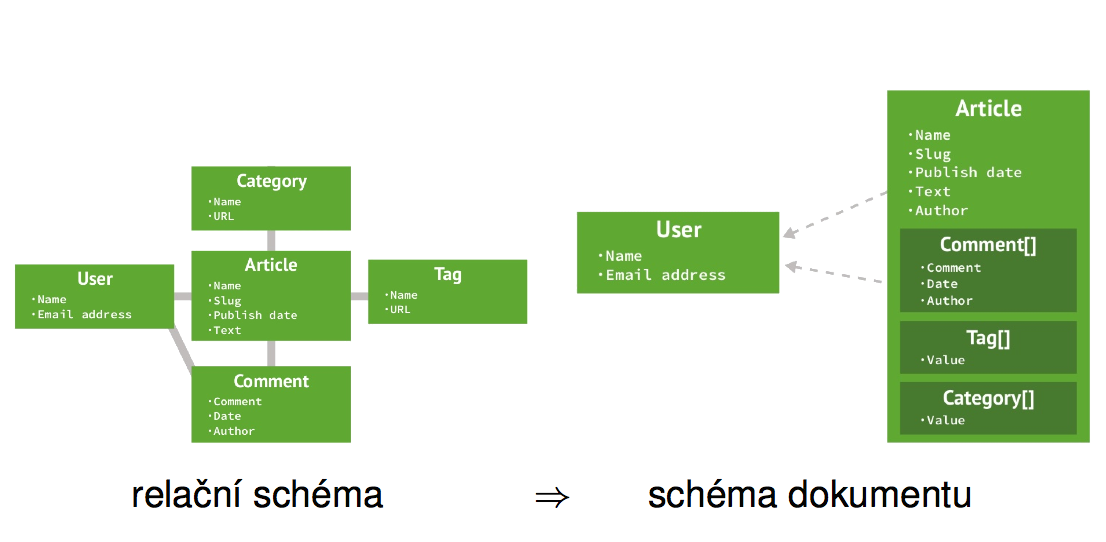
\includegraphics[scale=0.3]{obrazky/schema-vs-documents}
\par\end{centering}
\caption{Srovnání způsobu ukládání dat v MySQL a MongoDB databázích. \cite{nosqlSlides}}
\end{figure}

\subsection{Syntaxe}
Relační databáze MySQL používá dotazovací jazyk SQL, zatímco MongoDB dotazuje pomocí volání javascriptových metod. Rozdíl v syntaxi dotazů je velký, ale u NoSQL databáze MongoDB je možné vidět snahu o přiblížení se terminologii SQL serverů. Následující tabulka dobře ilustruje srovnání syntaxe databází MySQL a MongoDB.
\begin{table}[h]
\centering
    \caption{Porovnání syntaxe základních operací MongoDB vs. MySQL \cite{mongoMySQLMapChart}}
    \begin{tabular}{ |p{1.9cm}|l|l| }
    \hline
    \multicolumn{3}{|c|}{Srovnání syntaxe MySQL a MongoDB} \\ \hline
    Operace & MySQL & MongoDB \\ \hline
	Vytvoření tabulky & 
	\begin{lstlisting}
CREATE TABLE users (
 id int(11) NOT NULL 
 	AUTO_INCREMENT,
 user_id varchar(30),
 age int(11),
 status char(1),
 PRIMARY KEY (id)
)
 \end{lstlisting}
 & 
 \begin{lstlisting}
db.users.insert( {
  user\id: "abc123",
  age: 55,
  status: "A"
} ) 
 \end{lstlisting} 
 \\ \hline
	Přidání atributu &
	\begin{lstlisting}
ALTER TABLE users
ADD join_date DATETIME
	\end{lstlisting} &
	\begin{lstlisting}
db.users.update(
 { },
 {$set: {date:new Date()}},
 { multi: true })	
	\end{lstlisting}	
	 \\ \hline
	 Odstranění atributu &
	\begin{lstlisting}
ALTER TABLE users
DROP COLUMNT join_date 
	\end{lstlisting} &
	\begin{lstlisting}
db.users.update(
    { },
    { $unset:{join_date:""}},
    { multi: true })	
	\end{lstlisting}	
	 \\ \hline
	Vytvoření indexu &
	\begin{lstlisting}
CREATE INDEX
 idx_user_asc_age_desc ON
 users(user_id, age DESC)
	\end{lstlisting}
	&
	\begin{lstlisting}
db.users.ensureIndex( 
{ user_id: 1, age: -1 } )
	\end{lstlisting}
	\\ \hline
	Vložení dat &
	\begin{lstlisting}
INSERT INTO 
users(user_id, age, status)
VALUES ("bcd001",
        45,
        "A")	
	\end{lstlisting} &
	\begin{lstlisting}
db.users.insert(
   { 
   user_id: "bcd001",
   age: 45,
   status: "A" }
)
	\end{lstlisting} \\ \hline
	Získání dat &
	\begin{lstlisting}
SELECT user_id, status
FROM users
WHERE status = "A"	
	\end{lstlisting}
	&
	\begin{lstlisting}
db.users.find(
    { status: "A" },
    { user_id: 1,
      status: 1,
      _id: 0 })
	\end{lstlisting}
	\\ \hline
	Editace dat &
	\begin{lstlisting}
UPDATE users
SET status = "C"
WHERE age > 25	
	\end{lstlisting} &
	\begin{lstlisting}
db.users.update(
   { age: { $gt: 25 } },
   { $set: { status: "C" } },
   { multi: true }
)	
	\end{lstlisting} \\ \hline
	Odstranění dat &
	\begin{lstlisting}
DELETE FROM users
WHERE status = "D"	
	\end{lstlisting}
	&
	\begin{lstlisting}
db.users.remove({status:"D"})
	\end{lstlisting} 
	\\ \hline
    \end{tabular}
    \label{tab:porovnaniSyntaxe}
\end{table}

\FloatBarrier
\subsection{Podpora platforem}
MySQL je databáze vyvíjená v C++ a je dostupná na všech běžně používaných systémech včetně FreeBSD. MongoDB je vyvíjeno ve stejném jazyce a je dostupné pro Windows, Linux, Mac OS X a Solaris.

Databázové ovladače jsou dostupné pro všechny nejpoužívanější jazyky, PHP podporuje práci s MySQL nativně, podporu MongoDB je nutno doplnit rozšiřujícím modulem. Moduly pro MongoDB jsou dostupné pro .NET platformu, Javu, Ruby, Python, Perl a další jazyky.

\subsection{Možnosti migrace existujících aplikací}
I když se MongoDB prezentuje jako vhodná náhrada MySQL řešení, rozdíly v návrhu těchto dvou databází jsou tak velké,  že případná migrace již provozované aplikace by znamenala velké změny v jejím kódu. Pokud aplikace používá nějaký ORM \footnote{Object Relation Mapping - automatické mapování databázových tabulek do objektů jazyka aplikace.} framework, možnosti migrace se díky další abstraktní vrstvě zvyšují. Oblíbený ORM framework Doctrine totiž nabízí databázový ovladač i pro MongoDB. Tyto frameworky, které mapují objekty aplikace na dokumenty v MongoDB, se nazývají ODM - Object Document Mapping frameworky. Obecně lze ale říci, že MongoDB je dobrou volbou spíše pro nové aplikace, migrovat již provozovanou aplikaci se příliš nevyplatí. Jedinou situací, kdy by byla migrace nezbytná, je pokrytí opravdu velké zátěže na kterou už relační databázové řešení nestačí. V tuto chvíli pomůže distribuované řešení na bázi MongoDB.

\subsection{Nástroje}
Pro relační databázi MySQL existuje celá řada nástrojů včetně oficiální desktopové aplikace MySQL Workbench. Častěji se ale pro správu databáze používají webová rozhraní. Nejznámější z nich, phpMyAdmin je vyvíjen již od roku 1998 \cite{phpMyAdmin}. Mezi jeho alternativy patří SQLBuddy nebo Adminer. Nástrojů pro MongoDB rozhodně neexistuje takové množství jako pro MySQL, vzhledem k tomu jak nová technologie MongoDB je. 

Utility pro import a export dat databáze jsou součástí distribuce MongoDB serveru. Také existuje několik desktopových aplikací pro správu této databáze. Velmi kvalitní aplikací je MongoDB Management Service, která zprostředkovává správu databáze v cloudu, včetně nasazování databázových serverů a tvorby záloh. Nástroj UMongo,  sloužící také pro správu clusteru, je dostupný pro Linux, Windows i Mac OS X.  Mezi aplikace určené především k práci s daty, patří Mac OS X klient MongoHub nebo komerční řešení MongoVUE postavené na platformě .NET. Existuje i několik webových rozhraní, podporující MongoDB. Jedním z nich je i již zmiňovaný Adminer. Zajímavým nástrojem je také aplikace Edda, která slouží k vizualizaci logů z MongoDB databáze. Přehledné shrnutí nástrojů pro MongoDB lze nalézt na webu \emph{mongodb-tools.com}.

\subsection{Licencování}
Databáze MongoDB je dostupná pod licencí GNU AGPL v3.0, je tedy zdarma pro komerční i nekomerční účely. Mongo klient je distribuován pod licencí Apache.

Zdarma pro veškeré účely je i MySQL, distribuované pod licencí GPL. MySQL navíc nabízí i placenou komerční alternativu, kterou je ale nutné použít, pouze ve specifických případech použití, například pokud chceme MySQL server dodávat jako součást naší aplikace \cite{payMysql}.

\chapter{Praktická část}
V praktické části se tato práce zaměřuje především na porovnání výkonu klasických SQL databází s novými NoSQL databázemi. Nelze však porovnávat kteroukoliv NoSQL databázi s kteroukoli SQL databází, protože většina NoSQL řešení je navržena k provozu v zcela jiných oblastech webové aplikace, než se používají běžné SQL servery. Proto byly z těchto dvou přístupů vybráni dva zástupci, kteří se zpravidla používají ke stejnému účelu, tedy perzistentnímu ukládání dat\footnote{Trvalé úkládání důležitých (například uživatelských) dat.} webové aplikace.

Těmito zástupci jsou MongoDB ze světa NoSQL databází a MySQL ze světa SQL databází. Obě databázová řešení jsou postavena na podobných konceptech, dokumentace MongoDB dokonce přímo porovnává možnosti a syntaxi s SQL servery \cite{mongoMySQLMapChart}.
Databáze budou porovnány z hlediska výkonu základních operací, především rychlosti uložení a následného získání dat. Testy budou spouštěny paralelně ve více instancích zároveň, budou se snažit simulovat reálnou konkurenci připojených klientů, která je u dnešních webových aplikací běžná. 

Jednotlivé databázové servery byly provozovány lokálně kvůli relevantním výsledkům testů, které tak nebudou náchylné na problémy nebo případné výpadky připojení. Na základě provedeného měření bude rozhodnuto, zda-li je NoSQL databáze MongoDB opravdu rychlejší než MySQL a jaký přínos v rychlosti bude mít databázový cluster. Veškeré ukázky příkazů a kódu v práci jsou zaměřeny na UNIXové systémy, mohou však fungovat i na platformě Windows s určitými změnami. Mezi těmito dvěma platformami je velký rozdíl především v adresářové struktuře.
\section{Vybraná databázová řešení}
Jako nejvhodnější kandidát pro porovnávání s SQL databázemi, byla vybrána dokumentově orientovaná databáze MongoDB. Hlavním důvodem tohoto výběru je velmi podobné zaměření NoSQL databáze MongoDB. I když se v principu stále jedná o key-value databází, jednotlivé objekty databáze vystupují jako logické celky (kolekce), na které lze nahlížet analogicky jako na SQL tabulky. Databáze MongoDB dokáže sloužit pro ukládání prakticky jakýchkoliv dat, je ale často nasazována u webových aplikací jako přímá náhrada SQL serverů.

Ze světa SQL databází byla vybraná asi nejpoužívanější open source databáze MySQL, které je mezi vývojáři webových aplikací velmi oblíbená hlavně kvůli jednoduchosti nasazení a její obsluhy. Existuje velké množství frameworků a knihoven, které zjednodušují práci s SQL serverem. Tyto knihovny se snaží objektový přístup, používaný v logice aplikace, převést na relační přístup, který používá SQL databáze. Dokumentově orientované NoSQL databáze jako je MongoDB takové nástroje nepotřebují, slouží totiž přímo jako objektové úložiště.

\section{Metodika měření a očekávané výsledky}
Obě databáze budou porovnány z hlediska rychlosti zpracování databázových operací. Porovnávány budou časové úseky, které databázový server nebo cluster potřebuje na zpracování požadavku. Těmito požadavky bude například vložení velkého počtu dat najednou a jejich následné získání podle klíče nebo jiné podmínky. Získaná množina dat bude ještě zobrazena, tím pádem dojde k skutečnému získání celé vybrané množiny z databáze. Tento mechanismus je nutné doplnit proto, že databázové ovladače optimalizují práci s databází a většinou vrací pouze iterátor, přes který je nutné postupně získat a zobrazit získaná data po jednom řádku. Iterátor je návrhový vzor, který obsahuje data vždy právě jednoho řádku tabulky a umožňuje procházet prvky zpravidla pomocí metod \emph{next()} a \emph{previous()}. Často se používá jako obalovací objekt pro výsledek databázového dotazu. Tato operace se většinou nazývá \emph{SELECT + FETCH}.

Dále bude testována operace přidání indexu nad množinu dat, která je u obou databází velmi náročná. Práce s indexy navíc zablokuje databázové servery, které nemohou po dobu provádění příkazu, zpracovávat další požadavky. Doba zpracování indexační operace je závislá na velikosti dat, které jsou v kolekci uloženy, proto je velmi vhodné rozmyslet si indexy již při návrhu databáze, nicméně MongoDB by mělo i v tomto ohledu dosahovat vyšších rychlostí než MySQL. Poslední operací, která bude nad databázemi testována, je smazání jednoho nebo více záznamů.

Testovací prostředí je napsané v programovacím jazyce PHP. Měření probíhá pomocí porovnání systémového času serveru před provedenou operací a po ní pomocí PHP funkce \emph{microtime()}, která vrací UNIXový timestamp. \footnote{Počet sekund od 1.1.1970 00:00:00.}

\begin{lstlisting}[caption={Ukázka kódu provádějícího měření}]
$t=microtime(true);
doSomething();
$result=microtime(true)-$t;
\end{lstlisting}

Přesnost uvažovaného postupu měření je dostatečná, jak dokládá provedený test doby běhu funkce \emph{sleep(3)}, která na zadanou dobu uspí provádění programu. Tato operace, podle provedeného měření, trvala 3.0008780956268 sekundy. Prostředí pracuje s velkou množinou náhodně vygenerovaných dat, které nejdříve načte do paměti a poté s nimi dále pracuje. Kvůli velikosti testovacích dat je také nutné zvýšit maximální velikost paměti, kterou může PHP alokovat.

Testovací prostředí přistupuje k databázím pomocí tzv. databázových ovladačů. Tyto ovladače představují sadu tříd, sloužících k obsluze databázového serveru. Pro přístup k MongoDB se používá ovladač MongoClient, který je volně dostupný jako rozšíření do PHP a poskytuje všechny možnosti práce s databází. Rozšíření obsahuje třídy MongoClient, MongoDB, MongoCollection a MongoCursor, z nichž každá reprezentuje určitou část MongoDB databáze. Třída MongoCursor je obalující třída (iterátor), obsahující samotná data získaná z  databáze. Modul pro práci s MongoDB není standardní součástí PHP a je nutné jej doinstalovat. Na UNIXových systémech je instalace jednoduchá pomocí nástroje \emph{pecl}. Na Windows existují zkompilované DLL knihovny, které je třeba ručně přidat do konfigurace PHP pomocí příkazu \emph{extension} \cite{phpMongo}. 

\begin{lstlisting}[caption={Instalace MongoDB rozšíření do PHP na UNIXových systémech}]
sudo pecl install mongo
\end{lstlisting}
Obsluha standalone MongoDB databázového serveru se nijak neliší od obsluhy databázového clusteru, je tedy doporučováno začít s aplikací na jednom serveru a v případě úspěchu aplikace a tím pádem větší zátěže generované uživateli, nasadit MongoDB cluster.

Operace nad MySQL serverem budou realizovaný pomocí knihovny NotORM Jakuba Vrány, která poskytuje jednoduché rozhraní pro práci s MySQL databázovým serverem. Knihovna poskytuje třídy reprezentující jednotlivé části databáze a nabízí široké možnosti dotazování. Jedná se o tenkou knihovnu, pouze zjednodušující práci s SQL serverem tím, že automaticky generuje SQL dotazy. Vzhledem k jednoduchosti knihovny lze říci, že její použití nebude mít žádný nebo minimální vliv na výsledky provedených testů \cite{notOrm}. 

Výsledkem provedených testů budou časové údaje stejných operací se stejnými daty provedených nad SQL databází MySQL a NoSQL databází MongoDB. Tyto databáze budou spouštěny jako standalone servery, tedy v režimu kdy jeden server obstará veškerou obsluhu databáze. Testy budou poté pro doplnění spuštěny také na MongoDB databázovém clusteru. Každý test bude spuštěn paralelně pětkrát, výsledné časy testů budou vytvořeny prostým aritmetickým průměrem.
Lze předpokládat, že na testované konfiguraci bude nejrychlejší MongoDB standalone server, síla clusteru se projeví až při skutečném nasazení na fyzické servery a při velmi vysoké zátěži.

\section{Testovací data}
Testovacími daty této práce budou objekty reprezentující fiktivní uživatele nějaké společnosti.
Jedná se o vysoce strukturované data, obsahující většinu datových typů (řetězec, celé číslo, desetinné číslo, logická hodnota, datum, čas, pole apod.). Zároveň je v nich realizována většina vazeb, které musejí být u relačních databází řešeny dalšími tabulkami. Bylo vytvořeno několik SQL tabulek a několik tříd aplikační logiky v PHP pro účely tohoto testovaní. Do NoSQL databáze MongoDB je možné tyto objekty ukládat přímo.

\begin{lstlisting}[caption={Ukázka objektu testovacích dat (zkráceno)}]
  {
    "hash": "53e0b94367d25cf04192f656",
    "index": 0,
	...
    "email": "rosannewhitfield@medcom.com",
    "phone": "+1 (906) 497-3016",
    "address": "611 Ovington Court, Curtice, New York, 6257",
    "registered": "2014-05-30T05:04:03 -02:00",
    "latitude": 49.332297,
    "longitude": -131.785071,
    "tags": ["do",
	  ...
    ],
    "friends": [
      { "id": 0,
        "name": "Sonja Moses"
      },
	  ...
    ],
    "favoriteFruit": "banana"
  },
\end{lstlisting}
Soubor testovacích dat tvoří 4 sady náhodně generovaných objektů po 25 000 záznamech. Data jsou uložena ve formátu JSON. Testovací prostředí načítá jednotlivý dataset do paměti, pokud je třeba testovat více než 25000 objektů zároveň, lze pomocí příkazu \emph{nextDataset()} získat další dataset. Je tedy možné v testech pracovat až se 100 000 unikátními objekty. Objekty reprezentují fiktivní osoby zaměstnané v nějaké organizaci. Tyto objekty byly vygenerovány pomocí nástroje \emph{JSON - Generator}, který je volně dostupný na Internetu. Tento nástroj generuje JSON objekty podle zadaných kritérií, nebo vlastních funkcí napsaných v Javascriptu a výborně se hodí pro testovaní webových aplikací. 

\section{Testovací prostředí}
Výkonnostní testování databází bylo provedeno na osobním notebooku MacBook Air (mid 2013), který sice disponuje relativně nízkým výkonem, ale nabízí velmi rychlé SSD disky přimo napojené na sběrnici PCI Express. Díky velmi vysoké rychlosti diskových operací (až 700MB/s), lze v oblasti databází očekávat zajímavý výkon \cite{macDiskSpeed}. Jednoduchý MySQL server společně s jedním MongoDB serverem budou provozovány přímo v prostředí Mac OS X 10.9.2. Stejné testy byly provedeny i nad virtuálním MongoDB databázovým clusterem s 10 připojenými servery, spravovaným pomocí nástrojů Docker a VirtualBox v operačním systému Ubuntu.

Testovací prostředí je napsáno v PHP a testy se spouští pomocí obyčejného HTTP požadavku. V rámce lokálního Apache serveru běží PHP 5.4.21, které komunikuje s databázemi pomocí ovladačů. Podpora MySQL je dostupná v rámci rozšíření \emph{mysqli} 5.0.10, MongoDB  doplňuje \emph{mongo} extension ve verzi 1.4.5. Samotné testy jsou obyčejné PHP třídy, rozšiřující základního předka \emph{BPTestCase}, který přináší funkcionalitu měření. Každá z testovacích tříd je zaměřená na jiný typ databází, jednotlivé testy jsou v nich implementovány jako metody. Kvůli velkému objemu testovacích dat a časové náročnosti provedených testů, je třeba zvýšit maximální množství paměti, kterou může testovací prostředí použít. Zároveň je nutné vypnout časový limit provádění PHP skriptů. Tyto změny lze provést v konfiguraci PHP, nebo přímo v kódu pomocí volání funkce \emph{ini\_set()}.

\begin{lstlisting}[caption={Nutná konfigurace PHP prostředí}]
ini_set('max_execution_time', 0);
ini_set('memory_limit', '1024M');
\end{lstlisting}

Každá testovací třída také může obsahovat metodu \emph{beforeTests()}, která je vždy zavolána před začátkem testování. Tato metoda většinou provádí připojení a autentizaci do databáze. Testovací prostředí podporuje i metodu \emph{afterTests()}, která bude zavolána vždy po skončení všech testů. Tato metoda není v testech využita, protože odpojení od databáze a úklid provádějí PHP databázové ovladače automaticky. 

\begin{lstlisting}[caption={Ukázka HTTP požadavku který spustí test "insert1000Test" na třídě MongoTest}]
http://<url>/runner.php?class=MongoTest&test=insert1000Test
\end{lstlisting}

Testovací prostředí je spolu s testy dostupné na přiloženém CD.

\subsection{MySQL standalone server}
Prvním databázovým serverem testovaným v této práci byl MySQL server ve verzi 5.6.16. 
Databázový server MySQL je nejpoužívanější zdarma dostupnou variantou SQL serveru a druhou nejpoužívanější databází vůbec \cite{enginesRanking}. Tohoto umístění dosáhla díky jednoduchosti jejího nasazení, dobrému výkonu a především proto že se jedná o volně šiřitelnou databázi. Na rozdíl od komerčních řešení, MySQL dlouho nepodporovalo pohledy, triggery a uložené procedury. Tyto vlastnosti, spolu s mnoha dalšími, byly doplňeny až v posledních letech. Databázi vytvořila švédská společnost MySQL AB, později vlastněna firmou Sun Microsystems, která je dnes pod křídly Oraclu. Velmi často je nasazována jako hlavní databáze do webových PHP aplikací v kombinaci se servery Apache (tzv. LAMP \footnote{Linux, Apache, MySQL, PHP.}). MySQL server byl jeden z prvních produktů, který používal tzv. dvojí licencování. Databáze je totiž distribuována jednak pod svobodnou licencí GNU GPL v3, ale také pod placenou licencí zahrnující plnou podporu.

Server lze spustit ve formě daemonu \emph{mysqld} stejně jako MongoDB, ale častěji se spouští přímo v systému jako služba. Instalace je na linuxových systémech jednoduchá, například na Ubuntu a podobných systémem stačí stáhnout balíček \emph{mysql-server} \cite{mysqlUbuntu}. 
\begin{lstlisting}[caption={Instalace MySQL serveru na Ubuntu}]
sudo apt-get install mysql-server
\end{lstlisting} 
Příkaz výše nainstaluje MySQL server v Ubuntu a podobných linuxových systémech. Server pak lze řídit pomocí vestavěného nástroje \emph{mysqladmin} nebo utility \emph{service}  \cite{mysqlUbuntu}.

\vspace{0.5cm}

\begin{lstlisting}[caption={Restart MySQL serveru pomocí utility service}]
sudo service mysql restart
\end{lstlisting}
Ve výchozím nastavení MySQL server běží na portu 3306 a přihlašovacím jménem je \emph{root} bez zadaní hesla. Server je dostupný také pro platformu Windows ve formě zkompilovaného EXE souboru. Existuje celá řada webových aplikací pro správu MySQL serveru, mezi nejoblíbenější patří nástroj Adminer, od českého vývojáře Jakuba Vrány. Tyto aplikace poskytují rozhraní pro komplexní správu databáze od vytvoření tabulek, vkládání dat nebo správu indexů, až po programování databázových procedur.
\pagebreak
\subsection{MongoDB standalone server}
Konkurentem SQL databáze MySQL byla v této práci moderní dokumentově orientovaná databáze MongoDB ve verzi 2.6.4.
Tato databáze umožňuje vedle běhu v clusteru, také možnost běhu jako standalone server. To znamená, že jeden databázový server má na starosti veškeré činnosti spojené s obsluhou databáze. Je tedy možné celou databázi provozovat pouze na jediném serveru. Způsobem interakce se standalone servery nijak neliší od clusterů, je tedy možné spustit databázový cluster až později, podle nároků obsluhované aplikace. MongoDB standalone servery jsou doporučovány pro použití v malých aplikacích nebo k testovacím učelům.  Databáze je oblíbena mezi vývojáři Javascriptových aplikací, především ve světě Node.JS, tedy serverového Javascriptu. Často se také používá ve spojení s klientským Javascriptem, běžícím v prohlížeci uživatele. Oblíbená je hlavně proto, že ukládá dokumenty ve formátu JSON a dotazování probíhá pomocí Javascriptu. V tomto jazyce lze také psát databázové procedury \cite{mongoDocs} nebo \emph{MapReduce} agregace.

MongoDB server používá primárního daemona \footnote{Označení programu, který je spuštěn dlouhodobě a není v přímém kontaktu s uživatelem (na rozdíl od běžných aplikací).} nazvaného \emph{mongod}. Ten zpracovává požadavky, získává data a na pozadí provádí optimalizace datových struktur \cite{mongod}.
\begin{lstlisting}[caption={Spuštění MongoDB standalone serveru}]
mongod --name mongoServer --dbpath /data/db --logpath /data/logs --logappend 
\end{lstlisting}
Tento příkaz spustí standalone MongoDB server na výchozím portu 27017.  Každou instanci serveru je vhodné pojmenovat. K tomu slouží parametr \emph{--name}, je zvykem tento parametr používat hlavně v databázových clusterech, je ale dobré pojmenovat server vždy. Také je nutné přidělit místo na disku, tedy nastavit adresář, nad kterým bude databáze operovat. Cesta k němu se předává parametrem \emph{--dbpath}. Tento parametr není povinný, ale je dobré ho zadávat vždy. MongoDB se jinak totiž snaží o ukládání databáze na místě, z něhož byl server spuštěn. Dále je dobré, aby server nevypisoval do konzole, ale svoje hlášky logoval do souboru, umístěného na stejném místě jako soubory databáze. Příznak \emph{--logappend} řekne databázovému serveru, že má pokračovat v logu, místo vytvoření nového. MongoDB databázový server totiž ve výchozím stavu vždy začíná logovat do prázdného souboru. 

Proces \emph{mongod} přijímá celou řadu dalších parametrů, mezi ty zajímavé patří například \emph{--directoryperdb}, který zajistí ukládání každé databáze do vlastní složky, nebo \emph{--smallfiles}, který způbobí, že MongoDB bude používat menší soubory, čímž se sníží výpočetní náročnost obsluhy databáze. Tento příznak se používá hlavně při testovaní. Pomocí parametrů se nastavuje také replikace, příslušnost serveru k danénu replica setu se určuje parametrem \emph{--replSet}. Poté lze příznaky \emph{--master} a \emph{--slave} určovat role serverů. Lze dokonce nastavit i žurnálování diskových operací, kvůli lepší ochraně dat. Pro produkční nasazení je vhodné použít parametr \emph{--nohttpinterface}, který vypne webové administrační rozhraní určené pro testovací provoz \cite{mongod}. 

\subsection{MongoDB databázový cluster}
Pomocí stejné verze NoSQL databáze MongoDB, jako by provozován standalone server, lze provozovat také databázový cluster. Clustering se v MongoDB řídí pomocí parametrů daemonu \emph{mongod} \cite{mongod}.  

Pro účely této práce byl virtuální databázový cluster. Tento cluster běžel lokálně pomocí nástroje Vagrant a virtulizační platformy VirtualBox v prostředí Ubuntu 14.04. V něm byly vytvořeny aplikační kontejnery, které reprezentovaly jednotlivé servery zapojené do MongoDB databázového clusteru. Tyto aplikační kontejnery byly vytvořeny pomocí nástroje Docker a jedná se velmi tenké virtualizované servery, které jsou navzájem propojeny a komunikují ve virtuální síti. Tato komunikace probíhá pouze pomocí mapování portů, jednotlivé servery jsou tedy dostupné na stejné IP adrese a různých portech.

Celkem bylo do databázového clusteru zapojeno 10 serverů. O ukládání dat se staraly 3 replica sety \footnote{Dvojice serverů, které se navzájem replikují, jeden slouží jako hlavní a druhý jako záloha v případě výpadku.}, meta data distribuovaly 3 konfigurační servery a jeden server sloužil jako router. Veškerá komunikace databáze s okolním světem probíhá vždy přes tento server. Databázový router je vstupním bodem MongoDB clusteru, jeho IP adresu a port je nutné předat aplikaci, která bude s databází pracovat. V tomto virtuálním clusteru budou všechny servery naslouchat na portu 27017, který se dále mapuje na jednotlivé porty dle tabulky níže. V produkčním nasazení bývá zvykem odlišit porty podle typu serveru. Port, na němž bude server naslouchat, lze jednoduše specifikovat v příkazu, kterým se server spouští. V následující části bude předveden postup spuštění jednotlivých serverů zapojených do databázového clusteru, tyto servery musejí být ve stejné síti a být spuštěny v uvedeném pořadí. V některých typech síti je třeba jejich komunikaci povolit ve firewallech.
\begin{table}[h]
\centering
\caption{Přehled adres a portů serverů zapojených do MongoDB clusteru \label{tab:clusterServers}}
\begin{tabular}{ | l | l | l | l | }
\hline
ID kontajneru&Mapované porty&Jména serverů & Účel\\ \hline
a45a6a2e17ef&49168->27017/tcp&mongos1 & Databázový router\\ \hline            
5a5f6a2ddf4d&49167->27017/tcp&configservers3 & Konfigurační server\\ \hline     
e0966225679c&49164->27017/tcp&mongos3r2  & Shard 3 - Slave\\ \hline         
8379ecacfabc&49163->27017/tcp&mongos3r1  & Shard 3 - Master \\ \hline        
7e270dc33f7d&49162->27017/tcp&configservers2 & Konfigurační server\\ \hline      
8bd9c829fc1a&49159->27017/tcp&mongos2r2 & Shard 2 - Slave\\ \hline           
f70cc6aef893&49158->27017/tcp&mongos2r1 & Shard 2 - Master\\ \hline          
af3029018f65	&49157->27017/tcp&configservers1 & Konfigurační server\\ \hline     
2577ea487e24&49154->27017/tcp&mongos1r2 & Shard 1 - Slave\\ \hline         
532120a087cf&49153->27017/tcp&mongos1r1 & Shard 1 - Master\\ \hline 
\end{tabular}

\end{table}
\subsubsection{Konfigurační servery}
Konfigurační servery slouží k ukládání metadat, tedy pomocných informací o uložených datech, jejich struktuře a umístění. Každý konfigurační server uchovává kompletní kopii metadat celého databázového clusteru. Konfigurační servery jsou vždy dvakrát zálohovány, to znamená, že každý MongoDB databázový cluster musí obsahovat přesně 3 konfigurační servery, které pro produkční nasazení musejí být fyzické. Konfigurační servery by měly být spuštěny jako první \cite{mongoCluster}.

\begin{lstlisting}[caption={Spuštění MongoDB konfiguračního serveru na portu 27017}]
mongod --name configservers1 --configsvr --dbpath /data/configdb --port 27017
\end{lstlisting}
\subsubsection{Router}
Funkci databázový routeru v MongoDB obstarává proces \emph{mongos}, který obsluhuje celý cluster a vyřizuje požadavky na databázi. Tento server komunikuje s konfiguračními servery a poté posílá požadavky dál na jednotlivé shardy, které vrátí požadované data. U menších typů aplikací bohatě postačuje používat jen jeden databázový router, nicméně počet jejich instancí není omezen a vysokozátěžové aplikace většinou používají více těchto routerů. Každému databázovému routeru je nutné vždy explicitně uvést adresy všech tří konfiguračních serverů. Doporučuje se používat DNS názvy namísto IP adres, kvůli možnosti výměny serveru bez nutnosti změny konfigurace. Každý z těchto routerů musí obsahovat stejné nastavení konfiguračních serverů \cite{mongoCluster}.

\vspace{0.25cm}
\begin{lstlisting}[caption={Spuštění MongoDB routeru na portu 27017, se třemi konfiguračními servery}]
mongos --configdb configservers1.mongo.dev.docker:27017, configservers2.mongo.dev.docker:27017, configservers3.mongo.dev.docker:27017 --port 27017
\end{lstlisting}
\subsubsection{Shardy}
Data uložená v clusteru se uchovávají v tzv. shardech, což jsou databázové servery sloužící pouze k ukládání dat. K těmto serverům neexistuje žádná možnost přímého přístupu, zpracování dotazů realizuje router.

Shardy mohou existovat ve dvou provedeních. Základní provedení se nazývá \emph{standalone server} a jedná se o klasické MongoDB servery bez replikace. Druhou možností jsou tzv. \emph{replica sety}. Replica set je dvojice serverů ve vztahu Master - Slave, které se navzájem replikují. Mechanismus čtení dat realizují vždy master servery, slave slouží pouze jako záloha v případě výpadku hlavního serveru \cite{mongoCluster}. Cluster popisovaný touto prací bude používat 3 shardy každý obsahující jeden replica set, celkem tedy 6 datových serverů. 

\begin{lstlisting}[caption={Spuštění jednoho MongoDB shardu na portu 27017 zapojeného do replica setu set1}]
mongod --name mongos1r1 --dbpath /data/db --replSet set1 --port 27017
\end{lstlisting}

Vytvořené shardy je nutné ještě přidat do clusteru, aktualizovat metadata konfiguračních serverů a dát o nich vědět databázovému routeru.
Připojíme se tedy pomocí MongoDB klienta k databázovému routeru a přidáme shardy do clusteru.
K tomu slouží metoda \emph{sh.addShard()}. 
\begin{lstlisting}[caption={Nastavení MongoDB shardu na databázovém routeru}]
sh.addShard("set1/mongos1r1.mongo.dev.docker:27017");
sh.addShard("set2/mongos2r1.mongo.dev.docker:27017");
sh.addShard("set3/mongos3r1.mongo.dev.docker:27017");
\end{lstlisting}

Dále je nutné zapnout sharding samotné databáze, aby se data v našem clusteru ukládala po částech. V této práci se pracuje nad databází \emph{database}.

\begin{lstlisting}[caption={Zapnutí shardingu nad databází database v MongoDB}]
sh.enableSharding("database")
\end{lstlisting}

Poslední věcí, kterou je nutné provést, je zapnout sharding na úrovni kolekce. Každá kolekce bude rozdělena na jednotlivé části podle tzv. shard key. Výběr tohoto klíče ovlivňuje efektivitu rozdělování, zpravidla je však používán index nad \_id dokumentů, který zohledňuje datum a čas vytvoření a umožňuje tedy dělit kolekce podle staří dokumentů, v nich uložených. Pokud nastavujeme sharding na kolekci, která již obsahuje data, je nutné vytvořit shard key ručně pomocí příkazu \emph{ensureIndex()}. Prázdné kolekci bude shard key nastaven automaticky \cite{mongoCluster}.
\pagebreak

\begin{lstlisting}[caption={Nastavení MongoDB shardingu pro kolekci testData v databázi database podle indexu \_id typu hashed}]
sh.shardCollection("database.testData",{_id:"hashed"})
\end{lstlisting}
\subsubsection{Replica sety}
Je třeba dále nastavit ke každému master serveru v shardu jeho slave server, který zastoupí práci hlavního serveru, pokud dojde k jeho výpadku nebo poškození hardwaru. Připojíme se tedy pomocí MongoDB klienta k hlavnímu serveru shardu a provedeme přidání slave serveru.
\begin{lstlisting}[caption={Konfigurace MongoDB replica setu na Master serveru}]
rs.initiate()
rs.add("mongos1r2.mongo.dev.docker:27017")
rs.status()
\end{lstlisting}

\subsubsection{DNS}
Je všeobecně doporučováno provozovat v databázovém clusteru ještě DNS server, který překládá jména serverů na jejich IP adresy. Tento mechanismus umožňuje propojit členy clusteru pomocí jejich hostname \footnote{Identifikátor (jméno) počítače nebo serveru v počítačové síti.} nikoli podle IP adres. Díky tomu lze členy clusteru dynamicky obnovovat v případě poškození hardwaru bez změny v konfiguraci clusteru \cite{mongoCluster}.

\pagebreak
Zpracování dotazu na databázový cluster tedy začíná na databázovém routeru, který na základě metadat získá požadované dokumenty od některého z shardů. Komunikaci mezi členy databázového clusteru a aplikací popisuje schéma níže.
\begin{figure}[h]
\begin{centering}
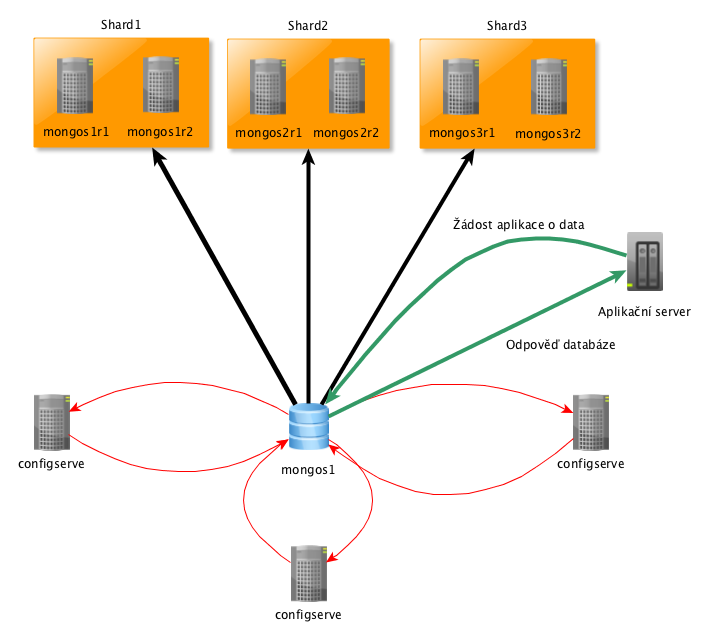
\includegraphics[scale=0.5]{obrazky/cluster-diagram}
\par\end{centering}
\caption{Schéma MongoDB databázového clusteru \label{fig:cluster-diagram}}
\end{figure}

\pagebreak
\section{Provedené testy}
Tato práce se pomocí otestování rychlosti databázových serverů pokusí rozhodnout, která z testovaných databází je vhodnější pro použití ve webové aplikaci. Vzájemně porovnávány budou relační databáze MySQL s NoSQL databází MongoDB. Porovnány budou časy zpracování základních operací s databází, tedy ukládání, editování a mazání dat. Také bude porovnán výkon těchto databází z hlediska práce s indexy. Testy indexace byly v práci zahrnuty proto, že se jedná u stávajících SQL řešení o velmi výpočetně náročnou operaci a bude zajímavé zjistit, zda-li tomu tak je i u NoSQL databází. 

Kompletní obsluhu testů zajišťuje PHP rozhraní napsané pro účely této práce, toto rozhraní má na starosti získávání náhodných dat, obsluhu databázových serverů, samotné testování a zobrazení výsledků. Samotnému testování tedy předchází ještě několik kroků.
Následující graf ukazuje jednotlivé kroky při testování a jejich podíly na celkové době běhu testu.
\begin{figure}[h]
\begin{centering}
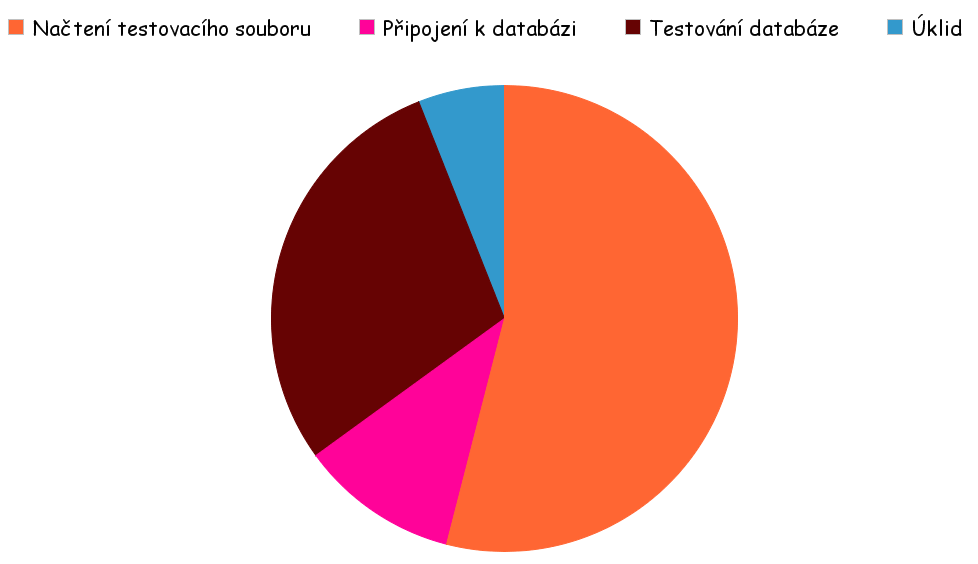
\includegraphics[scale=0.3]{obrazky/runtime-graf}
\par\end{centering}
\caption{Graf podílů jednolivých kroků při testování.\label{fig:runtimeGraph}}
\end{figure}
\FloatBarrier
Každý databázový dotaz byl před zahájením testování 5x zavolán nanečisto. Je to proto, že databázové servery provádějí optimalizace dat i za běhu a doba zpracování prvních několika dotazů bývá větší, než těch následujících.
\subsection{Ukládání dat}
Provedené testy ukládání dat simulují vytváření nových uživatelů v prostředí webové aplikace. Bylo testováno uložení 1000, 10 000 a 100 000 objektů, reprezentující fiktivní zaměstnance v organizaci. Výsledné časy jsou průměrem odezvy pěti paralelně spuštěných testů nad prázdnými databázemi.

K vkládání dat v MySQL slouží příkaz \emph{INSERT INTO} o specifické syntaxi, NoSQL databáze MongoDB používá funkci \emph{insert()}. Tato metoda přímo přijímá objekt, při testech bylo tedy možné použít rovnou objekty testovacích dat. Při testování MySQL bylo nutné vytvořit datový model, podle kterého budou data ukládaná do tabulek.
\begin{figure}[h]
\begin{centering}
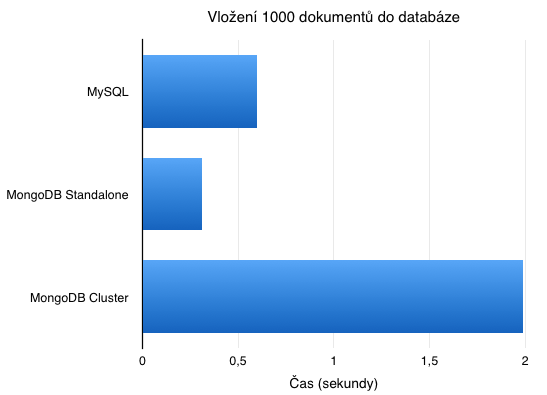
\includegraphics[scale=0.5]{obrazky/grafy/insert1000}
\par\end{centering}
\caption{Graf ilustrující dobu uložení 1000 záznamů do databáze}
\end{figure}

Jak je vidět na grafu výše, v uložení 1000 záznamů byla rychlejší databáze MongoDB. Zvládla tyto záznamy uložit za méně než půl vteřiny, naproti tomu MySQL potřebovala asi 0,7 sekundy. Cluster v testech zaostával, vzhledem k jeho virtualizované podobě nemůže konkurovat standalone variantám. Síla clusteru by se projevila až při skutečném provozu na fyzických serverech.

\begin{figure}[h]
\begin{centering}
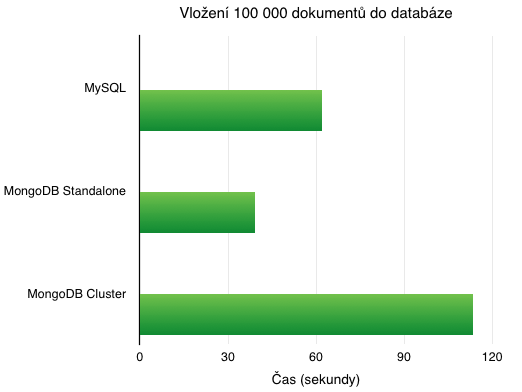
\includegraphics[scale=0.5]{obrazky/grafy/insert100k}
\par\end{centering}
\caption{Graf ilustrující dobu uložení 100 000 záznamů do databáze}
\end{figure}

Tento graf znovu dokazuje fakt, že NoSQL databáze dokáže rychleji ukládat data než MySQL. Jak je vidět, i při ukládání většího objemu dat je nejpomalejší clusterové řešení.
\subsection{Získávání dat}
Testy získávání dat si kladly za cíl simulovat situaci nalezení dané osoby v databázi a to buď přímo, za pomocí unikátního identifikátoru, nebo pomocí nějakých jeho vlastností (charakteristik). Dotazování podle unikátního identifikátoru by z principu mělo být rychlejší. V MySQL slouží k dotazování příkaz \emph{SELECT}, který nejdříve definuje tabulky a jejich sloupce, která chce získat a poté pomocí klauzule \emph{WHERE} definuje vyhledávací kritéria. MongoDB používá opačný přístup. Získávání dat probíhá pomocí funkce \emph{find()}, která v prvním parametru očekává vyhledávací kritéria. Tyto kritéria tvoří objekt, jehož atributy jsou dvojice reprezentující očekávanou hodnotu v dané vlastnosti (například \{age: 25\}). Mezi těmito atributy objektu platí logické AND. Druhým parametrem funkce find je tzv. projekce, což je objekt obsahující výčet těch atributů dotazových objektů, které mají být získány. Obě databáze tedy disponují stejnými mechanismy jen s drobnými odchylkami v syntaxi. Dotazování probíhalo nad množinou jednoho milionu záznamů.

\begin{figure}[h]
\begin{centering}
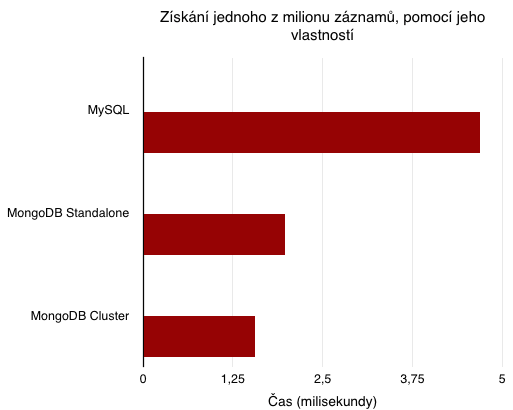
\includegraphics[scale=0.6]{obrazky/grafy/select}
\par\end{centering}
\caption{Graf ilustrující dobu nutnou pro získání jednoho záznamu pomocí jeho vlastností}
\end{figure}

\pagebreak
V oblastí získávání dat je tentokrát nejrychlejší MongoDB cluster a to i navzdory faktu, že je provozován virtuálně. Ale i varianta standalone serveru byla asi o polovinu rychlejší než MySQL. Relační databáze potřebovala k získání jednoho z milionu záznamů téměř 5 milisekund. Rozdíl mezi  získáním dat pomocí unikátního identifikátoru a pomocí vlastností daného objektu, je u NoSQL databáze zanedbatelný.  MongoDB dokáže získat záznam podle jeho klíče průměrně za 1,81 ms, zatímco podle jeho vlastností na to databáze potřebuje necelé 2 milisekundy. U relační databáze MySQL je situace odlišná. Na získání záznamu podle primárního klíče potřebuje asi 2ms, ale podle jeho vlastností téměř 5ms. Rozdíl ve rychlosti těchto dvou operací je tedy, v případě SQL databáze MySQL, značný.

\begin{lstlisting}[caption={Ukázka dotazu na osobu pomocí charakteristik v MongoDB}]
db.testData.find({
	gender:'male',
	tags:'elit',
	$or:[
		{age:{
				$gte:30
			}},
		{isActive:false}
		]
	})
\end{lstlisting}

Tento dotaz představuje ukázku složitějšího dotazování podle hodnot v daných polích. Výsledkem tohoto dotazu budou všichni muži, kteří jsou v elitní sekci a je jim buď více než 30 let, nebo již nejsou aktivní. 

Zvlášť byly testovány operace samotného dotazu na databázi (SELECT) a kompletního získání dat z databáze (SELECT + FETCH). Jednotlivé časy jsou průměrem z pěti paralelních testování. Získání dat je totiž jen jednou z částí manipulace s databází, je také nutné data načíst do struktur jazyka aplikace. Této operací se říká \emph{SELECT \& FETCH}. Testovací prostředí, použité v této práci, načítá data do PHP polí. Výsledek tohoto testu by měl být stejný jako výsledek obyčejného testu získání dat, protože samotné získání dat je nedílnou součástí tohoto testu. Z grafu níže lze potvrdit dominanci dokumentově orientované databáze MongoDB.
\begin{figure}[h]
\begin{centering}
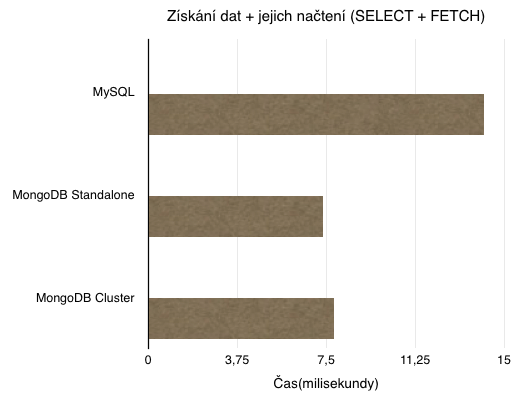
\includegraphics[scale=0.6]{obrazky/grafy/selectfetch}
\par\end{centering}
\caption{Graf ilustrující dobu nutnou pro získání jednoho záznamu pomocí jeho vlastností včetně následného načtení do struktur aplikace}
\end{figure}

\FloatBarrier
\subsection{Editace}
Další důležitou databázovou operací je editace dat, v MySQL realizovaná pomocí příkazu \emph{UPDATE}. Za tímto příkazem jsou u SQL serverů definovány změny pomocí klauzule \emph{SET}, následovanou klauzulí WHERE s vyhledávacími kritérii. NoSQL databáze obecně chápou editaci dat trochu jinak. Pohlížejí na ni jako na nahrazení jednoho objektu jiným, MongoDB k tomu nabízí funkci \emph{update}. Tato funkce očekává jako první parametr již známý objekt s vyhledávacími kritérii, druhý parametr tvoří objekt, nahrazující ten nalezený. Druhou možností je použití speciálního operátoru \emph{\$set}, který umožňuje klasickou částečnou editaci stejnou jako nabízejí SQL servery prostředníctvím příkazu \emph{UPDATE}. Tento operátor se předává v objektu v třetím parametru funkce. Zde se také pomocí operátoru \emph{\$multi} povoluje editace více dokumentů najednou.

\begin{figure}[h]
\begin{centering}
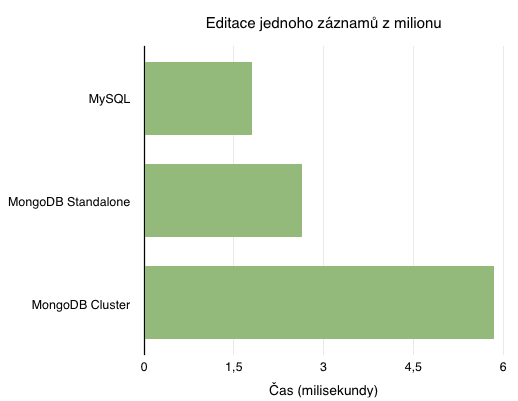
\includegraphics[scale=0.5]{obrazky/grafy/update}
\par\end{centering}
\caption{Graf ilustrující dobu nutnou pro editaci jednoho záznamu z testovací množiny}
\end{figure}
\FloatBarrier
Na grafu výše je patrné, že tentokrát byla rychlejší relační databáze MySQL, modifikace dat je také jednou z oblastí kde v tomto testování zvítězila. Je to především proto, že relační databáze MySQL je na úpravu uložených dat lépe navržena, zatímco dokumentově orientovaná databáze MongoDB s úpravami již jednou uložených objektů příliš nepočítá. Jak již bylo zmíněno, k dosažení možností editace podobné SQL příkazu \emph{UPDATE} je nutné využít operátor \emph{\$set}.

\begin{lstlisting}[caption={Ukázka editace záznamu za pomocí operátoru \$set v MongoDB}]
db.testData.update({_id:ObjectId('53e5fcaf37947b4210d69ca2')},
{$set:{index:25,isActive:true,favoriteFruit: 'apple'}})
\end{lstlisting}

\subsection{Práce s indexy}
Indexy slouží k rychlejšímu prohledávání databáze a zajišťují určité stavy sloupce napříč tabulkou. Nastavují se na parametrech objektu (MongoDB) nebo na sloupci v tabulce (MySQL). Indexy v MySQL urychlují provádění WHERE operací, poskytují záruky unikátnosti sloupce nebo umožňují fulltextově vyhledávat. Index můžeme definovat pomocí příkazu CREATE INDEX.

\begin{lstlisting}[caption={Ukázka vytvoření indexu v MySQL}]
CREATE INDEX IDX_ZAMESTNANEC_BYDLISTE
ON Zamestnanci (ulice, mesto, psc); 
\end{lstlisting}

Dokumentově orientovaná databáze MongoDB používá indexy pro urychlení přístupu k datům nebo implementaci shardingu (dělení databáze). Unikátní indexy jsou také podporovány. Ke správě indexace se v MongoDB používá metoda \emph{ensureIndex()}, která jako první přijímá objekt s definicemi indexů a jejich typů, druhým parametrem lze specifikovat typ indexu a další parametry indexace. Indexy se v MongoDB nastavují pro právě jednu kolekci.

\begin{lstlisting}[caption={Ukázka vytvoření unikátního indexu pro login v MongoDB}]
db.testData.ensureIndex({login:1},{unique:true})
\end{lstlisting}

Vzhledem ke výpočetní složitosti indexace je všeobecně doporučováno vytvářet indexy v momentě vzniku kolekce nebo tabulky, často je ale potřeba přidat nový index do kolekce,
která obsahuje data. Těch dat může být velké množství a doba vytvoření nového indexu je závislá na jejich velikosti. V rámci tohoto testování budou přidávány indexy na množinu jednoho miliónu záznamů. 

\begin{figure}[h]
\begin{centering}
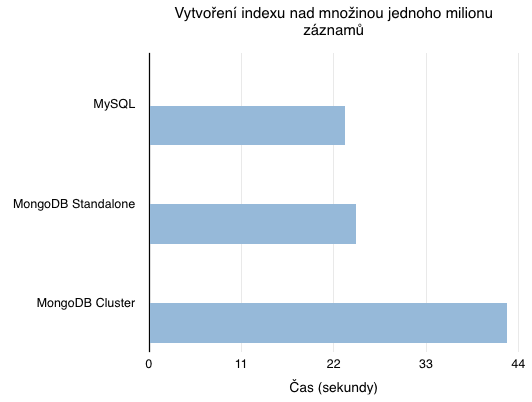
\includegraphics[scale=0.6]{obrazky/grafy/addindex}
\par\end{centering}
\caption{Graf ilustrující dobu nutnou pro vytvoření indexu nad množinou milionu záznamů}
\end{figure}
Práce s indexy představuje druhou oblast, kde v tomto testování zvýtězila relační databáze MySQL. Bylo testováno vytvoření indexu o dvou sloupcích na testovací množině jednoho miliónu záznamů. MySQL tuto úlohu zvládlo průměrně za 23,3s, NoSQL databáze MongoDB byla asi o vteřinu pomalejší a databázový cluster na tuto úlohu potřeboval téměř 44 sekund.

\subsection{Mazání dat}
Poslední operace s daty, které ještě nebyla testována, je jejich odstraňování. Mazání záznamů z databáze probíhalo na základě jejich unikátního identifikátoru, který byl náhodně vybrán z testovací množiny jednoho milionu záznamů.
\begin{figure}[h]
\begin{centering}
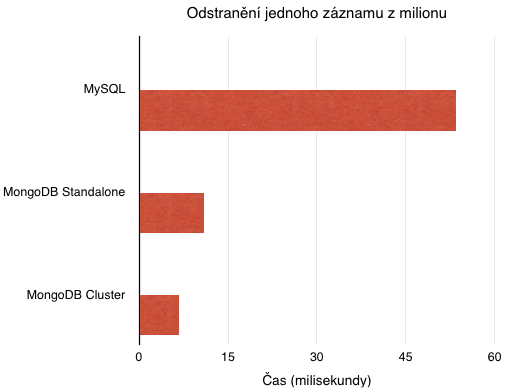
\includegraphics[scale=0.6]{obrazky/grafy/delete}
\par\end{centering}
\caption{Graf ilustrující dobu nutnou pro smazání jednoho záznamu z testovací množiny}
\end{figure}

V tomto případě úlohu nejlépe zvládl databázový cluster. Operace odstranění dat je dobrou ukázkou výhod clusteru, díky rozdělení dat na menší bloky, je v nich možné vyhledávat rychleji. Relační databáze MySQL, ukládající všechna data na jedno místo, na tuto úlohu potřebovala téměř 55 milisekund, zatímco databázový cluster jen asi 6 ms. Standalone varianta MongoDB databáze to zvládla za necelých 11 ms.

\chapter{Vyhodnocení výsledků}
Cílém této práce bylo rozhodnout, která ze dvou vytyčených databází je tou lepší pro použití ve webové aplikaci jako hlavní úložiště dat. Byly otestovány všechny operace, které jsou v moderní webové aplikaci očekávané od databázového serveru. Bohužel nelze na základě provedeného měření jednoznačně prohlásit, která z databází je pro tento účel vhodnější. Ačkoli byla NoSQL databáze MongoDB ve většině případů rychlejší než MySQL, rozdíl mezi nimy rozhodně nebyl propastný. MySQL bylo pomalejší v ukládání a získávání dat, naopak editaci dat mělo vyřešenu lépe. Úlohy získání nebo vymazání dat z velké testovací množiny miliónu záznamů zase nejrychleji zvládl MongoDB databázový cluster. Parelelní testovaní totiž nedělalo clusteru sebemenší problém. Rychlost indexace dat jednotlivých databází je velmi podobná, zde jsou rozdíly v řádu jednotek milisekund. Zajímavým faktem, který byl nameřen, je rozdíl v rychlosti těchto databází při mazání jednoho záznamu z velké množiny dat.
Relační databáze MySQL byla v tomto případě asi 5x pomalejší než MongoDB při použití standalone serveru. MongoDB cluster byl ještě rychlejší. Výsledky všech testů lze nálézt v přílohách této práce, testovací prostředí a testy samotné se nacházejí na přiloženém CD.

Velkým plusem databáze MongoDB je distribuovaný návrh. Dobře se hodí pro použití v nově vznikajících aplikacích, kde nabízí flexibilitu datových modelů a schopnost dobře reagovat na zvyšování záteže webové aplikace. Z provedených testů vyplývá, že rozdíly v rychlosti těchto databází jsou nízké, pokud si tedy vznikající webová aplikace vybere MySQL, získá veškeré schopnosti dotazovacího jazyka SQL spolu s dobrou rychlostí odezvy a dostatečným výkonem. Očekává-li se v aplikaci  velká zátěž nebo bude-li potřeba provádět operace nad velkou množinou dat, měla by webová aplikace použít některé z NoSQL řešení. Tato práce doporučuje použití dokumentově orientované databáze MongoDB při vývoji nové webové aplikace. Jedná se o moderní, výkonnou a dynamicky se rozvíjející databázi, která aplikaci nebude omezovat ani v případě velkého zájmu uživatelů. Velké odlišnosti v návrhu a datových modelech v  MongoDB však prakticky znemožňují jednoduchou migraci již existující aplikace, postavené na relačním řešení.



\chapter{Závěr}
V práci byly představeny NoSQL databáze jako nová databázová řešení, sloužící pro specifický druh využití, ale i jako náhrada relačních SQL databází. Byly představeny hlavní výhody NoSQL databází, jejich specifické vlastnosti a funkcionality. Práce popsala hlavní zástupce těchto databází a srovnala jejich možnosti použití v reálných webových aplikacích. Bylo provedeno porovnání NoSQL databáze MongoDB a SQL databáze MySQL, které se často používají ke stejnému účelu, tedy jako databáze pro webovou aplikaci, ukládájící objekty podle jejich typu. Klasické tabulky, známe z relačních databází v MongoDB představují kolekce. Tyto databáze byly nejprve srovnány teoreticky, podle jejich terminologie, syntaxe nebo reprezentace uložených dat. V praktické části byly provedeny výkonnostní testy těchto databází. Na základě těchto testů nebylo rozhodnuto, která databáze je opravdu lepší, byť v rychlosti zpracování většinou zvítězila NoSQL databáze MongoDB. 

NoSQL databáze neměly a ani nemají sloužit jako náhrada klasických relačních SQL databází, to ale nikdy nebyl ani jejich účel. První implementace vznikaly přímo na míru potřebám projektů, na kterých byly poté nasazeny, přímo na řešení určitých problémů, které vyvstaly. Hlavním důvodem jejich vzniku byla potřeba rychle a efektivně pracovat s obrovským množstvím dat. I proto byly průkopníky v této oblasti hlavně velké internetové firmy jako je Google nebo Facebook, které nedokázaly se svými obrovskými datovými objemy dobře pracovat pomocí tehdy dostupných technologií. Postupem času se našly další oblasti, kde  mohly NoSQL databáze najít své uplatnění. Rychlých key-value úložišť se začalo ve velkém využívat k ukládání velkého množství jednoduchých dat, velmi často jen například jedinečných idetifikátorů sezení pro každého přihlášeného uživatele. Dokumentově orientované databáze jsou vhodné pro strukturované ukládání nestejných dat. Jedná-li se o velké množství stejných dat, je výhodnější použít sloupcově orientovanou databázi. Grafové NoSQL databáze se zase velmi dobře hodí pro ukládání dat majících velké množství vazeb.

NoSQL databáze našly svá uplatnění, stejně jako ho našly klasické relační databáze a je jasné, že oba dva přístupy k ukládání a správě dat mohou existovat společně a je velmi těžké rozhodnout, který je ten „lepší“. Každý z těchto přístupů je má své výhody a nevýhody. MySQL přináší jednoduchý provoz, konzistenci dat a dotazovací jazyk SQL. MongoDB nabízí volnost podoby ukládaných dat a výborné možnosti škálování výkonu. Je na vývojářích, aby rozhodli která z těchto databází bude vhodnější pro použití v jejich aplikaci. Úkolem této práce bylo přinést srovnání dvou zcela odlišných databází, jejichž oblasti využití se překrývají.  

\section{Další směry výzkumu v oblasti}
Třetím testovacím prostředím, použitým v této práci, byl MongoDB databázový cluster. Ačkoli byl cluster ve většině testů pomalejší než MongoDB standalone server, a to z hlavně z důvodu virtualizace celého clusteru, bylo by zajímavé spustit provedené testy ještě na skutečném fyzickém clusteru. Potom by pravděpodobně MongoDB cluster zvítězil ve všech ohledech. Také by bylo možné do testů zařadit i MySQL Galera Cluster, tedy technologii pro distribuovaný běh relační databáze MySQL.

NoSQL databáze jsou velmi rozsáhlým tématem, existují desítky různých NoSQL databázových serverů, určených k obsluze různých typů dat. Zajímavým směrem vhodným pro další výzkum je tzv. \emph{Polygnot Persistance}. Tento koncept podle Martina Fowlera popisuje nasazení více databázových systémů zároveň pro různé druhy dat. Fowler udává, že pro každý typ dat je vhodné jiné prostředí, jiný jazyk a jiná databáze \cite{fowlerpp}. To znamená, že vedle sebe beží klasická relační databáze (na obrázku jako RDBMS), grafová databáze, dokumentově orientovaná databáze a další. Každá z těchto databází ukládá specifický typ dat, pro který je navržena nejlépe. Na obrázku níže jsou vidět různé databáze a jejich způsob využití ve fiktivní aplikaci. Je zde dobře vidět jak se mohou NoSQL databáze výborně doplňovat s relačními SQL databázemi.
\begin{figure}[h]
\begin{centering}
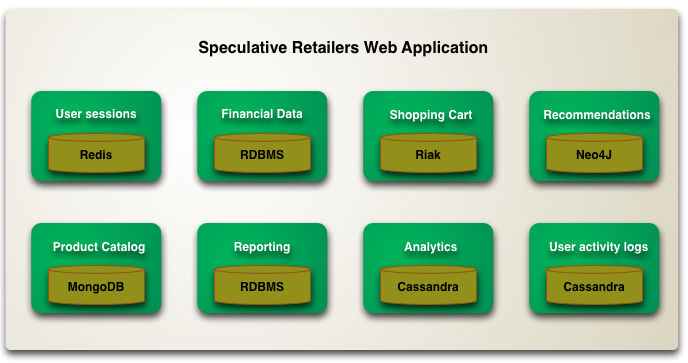
\includegraphics[scale=0.45]{obrazky/polygnot-persistance}
\par\end{centering}
\caption{Ukázka typů dat a jejich databází ve fiktivní aplikaci podle konceptu Polygnot Persistance \cite{fowlerpp}}.
\end{figure}

\addcontentsline{toc}{chapter}{Literatura} 
\begin{thebibliography}{10}
\bibitem{cassandra} LAKSHMAN, Avinash; MALIK, Prashant. \emph{Cassandra: a decentralized structured storage system} ACM SIGOPS Operating Systems Review, 2010, 44.2: 35-40.
\bibitem{redisBenchmark} Redis, \emph{Benchmarking Redis} {[}online] {[cit 19.6.2014]} Dostupné z WWW: \url{https://code.google.com/p/redis/wiki/Benchmarks}
\bibitem{nosqlBenchmark} Moredevs. \emph{MySql vs MongoDB performance benchmark} {[}online] {[cit 15. Červenec 2014]} Dostupné z WWW: \url{http://www.moredevs.ro/mysql-vs-mongodb-performance-benchmark/}
\bibitem{gunzl}GÜNZL, Richard. \emph{NoSQL databáze}. Praha, 2012. Bakalářská práce. Vysoká škola ekonomická v Praze.
\bibitem{peteraMongo}PETERA, Martin. \emph{MongoDB}. Praha, 2013. Bakalářská práce. Vysoká škola ekonomická v Praze.
\bibitem{strauchNosql} STRAUCH, C. \emph{NoSQL Databases}. Stuttgart 2011. Diplomová práce. Stuttgart Media University {[}online] {[cit 20. Červenec 2014 ]}. Dostupné z: \url{http://www.christof-strauch.de/nosqldbs.pdf}
\bibitem{panykoNosql} PANYKO, Tomáš. \emph{NoSQL databáze}. České Budějovice 2013. Bakalářská práce. Jihočeská univerzita v Českých Budějovicích.
\bibitem{coddSql}CODD, Edgar F. \emph{A relational model of data for large shared data banks}. Communications of the ACM, 1970, 13.6: 377-387.
\bibitem{sqlDatabaze}SKŘIVAN, Jaromír. \emph{Databáze a jazyk SQL} {[}online] {[cit. 20. Srpen 2013]} Dostupné z WWW: \url{http://interval.cz/clanky/databaze-a-jazyk-sql/}
\bibitem{nosqlDistilled} SADALAGE, Pramod J.; FOWLER, Martin. \emph{NoSQL distilled: a brief guide to the emerging world of polygnot persistence.} Pearson Education, 2012.
\bibitem{mysqlDataTypes}Oracle Corporation. \emph{MySQL 5.0 Reference Manual, Chapter 11: Data Types} {[}online] {[cit. 29. Srpen 2013]} Dostupné z WWW: \url{http://dev.mysql.com/doc/refman/5.0/en/data-types.html}
\bibitem{acid} CHAPPLE Mike, \emph{The ACID Model} {[}online] {[cit.2. Září 2013]} Dostupné z WWW: \url{http://databases.about.com/od/specificproducts/a/acid.htm}
\bibitem{transactions} LEWIS, Philip M.; BERNSTEIN, Arthur J; KIFER, Michael. \emph{Databases and transaction processing: an application-oriented approach} Addison-Wesley 2002
\bibitem{pesimistic_optimistic} JABR Mohammad. \emph{Differences between Pessimistic and Optimistic Locking} {[}online] {cit. 3. Září 2013} Dostupné z WWW: \url{http://mjabr.wordpress.com/2011/06/10/differences-between-pessimistic-and-optimistic-locking/}
\bibitem{oracle_transactions} Oracle Corporation. \emph{Oracle Database Concepts 11g Release 1 (11.1)} {[}online] {[cit. 10. Září 2013]} Dostupné z WWW: \url{http://docs.oracle.com/cd/B28359_01/server.111/b28318/transact.htm}
\bibitem{galeracluster} Codership Ltd. \emph{Galera cluster documentation} {[}online] {[cit 30.7.2014]} Dostupné z WWW: \url{http://galeracluster.com/documentation-webpages/}
\bibitem{strozziNoSQL}STROZZI, C. \emph{A Relational Database Management System} {[}online] {[cit. 21. Srpen 2013]} Dostupné z WWW: \url{http://www.strozzi.it/cgi-bin/CSA/tw7/I/en_US/NoSQL/Home%20Page}
\bibitem{augiNoSQL}AUGUSTÝN, Michal. \emph{Zamyšlení nad NoSQL. Augiho web} {[}online] {[cit 20. Srpen 2013]} Dostupné z WWW: \url{http://www.augi.cz/programovani/zamysleni-nad-nosql/}
\bibitem{cattellStores}CATTELL, Rick. \emph{High Performance Scalable Data Stores.} {[}online] {[cit 20. Srpen 2013]} Dostupné z WWW: \url{http://cattell.net/datastores/Datastores.pdf}
\bibitem{mongoConsist}10gen, inc. \emph{MongoDB - On distributed consistency}. MongoDB. {[}online] {[cit 28. Srpen 2013]} Dostupné z WWW: \url{http://blog.mongodb.org/post/498145601/on-distributed-consistency-part-2-some-eventual}
\bibitem{gilbertCap} GILBERT, Seth.; LYNCH Nancy. \emph{Brewer’s Conjecture and the Feasibility of Consistent, Available, Partition-Tolerant Web Services} {[}online] {[cit 30. Srpen 2013]}Dostupné z WWW: \url{http://lpd.epfl.ch/sgilbert/pubs/BrewersConjecture-SigAct.pdf}
\bibitem{cap} SIMON, Salomé. \emph{Brewer's CAP Theorem} {[}online] {[cit 30. Srpen 2013]} Dostupné z WWW: \url{https://www.cs.unibas.ch/fileadmin/Lectures/HS2012/CS341/workshops/reportsAndSlides/ReportSalomeSimon.pdf}
\bibitem{nosqlSlides} RYCHLÝ, Marek; KOLÁŘ Dušan. \emph{NoSQL databáze - Přednáška pro PDB} 2013, Vysoké učení technické v Brně, Fakulta informačních systémů {[}online] {[cit 1. Srpen 2014]} Dostupné z WWW: \url{http://www.fit.vutbr.cz/~rychly/public/docs/slides-nosql-databases/slides-nosql-databases.print.pdf}
\bibitem{beltrameKeyValue} BELTRAME, Carlo. \emph{Key-value stores} Algorithms for Database Systems Seminar, 2013 {[}online] {[cit 27. Srpen 2013]} Dostupné z WWW: \url{http://www.ifi.uzh.ch/dbtg/teaching/courses/SDBS/Beltrame.pdf}
\bibitem{redisDocs} Redis \emph{Redis Documentation} {[}online] {[cit 27. Srpen 2013]} Dostupné z WWW: \url{http://redis.io/documentation}
\bibitem{tolitStorelist}TOLITIUS, Anatoly. \emph{Key Value Store List} {[}online] 2009 {[cit 25. Srpen 2013]} Dostupné z WWW: \url{http://www.dotkam.com/2009/08/30/key-value-store-list/} 
\bibitem{enginesRanking}Db engines. \emph{Ranking.} {[}online] {[cit 1. Srpen 2014]} Dostupné z WWW: \url{http://db-engines.com/en/ranking}
\bibitem{mongoDocs} MongoDB, Inc. \emph{The MongoDB 2.6 Manual} {[}online] {[cit. 1. Srpen 2014]} Dostupné z WWW: \url{http://docs.mongodb.org/manual/}
\bibitem{changBigtable}CHANG, F. et al. \emph{Bigtable: A distrubuted Storage System for Structured Data} {[}online] 2006. {[cit 27. Srpen 2013]} Dostupné z WWW: \url{http://static.googleusercontent.com/media/research.google.com/cs//archive/bigtable-osdi06.pdf}
\bibitem{regnerVse}REGNER, Tomáš. \emph{Dokumentově orientované open source databázové systémy} Praha, Vysoká škola ekonomická v Praze, 2012.
\bibitem{columnDB} ABADI, D.; BONCZ, S.; HARIZOPOULOS, S.; IDREOS S.; MADDEN S. \emph{The Design and Implementation of Modern Column\-Oriented Database Systems} 2013, Foundations and Trends in Databases 5, Dec 2013, 198-280
\bibitem{graphDb}ROBINSON, Ian a kol.\emph{Graph Databases}. O'Reilly, 2013. ISBN 978-1449356262.
\bibitem{neo4j}Neo Technology, Inc. \emph{Neo4j documentation} {[}online] {[cit 2. Říjen 2013]} Dostupné z WWW: \url{http://www.neo4j.org/learn/}
\bibitem{cypher} Neo Technology, Inc. \emph{Cypher Query Language}. {[}online] {[cit 2. Říjen 
2013]} Dostupné z WWW: \url{http://docs.neo4j.org/chunked/milestone/cypher-query-lang.html}
\bibitem{neo4jLicence} Neo Technology, Inc. \emph{Neo4j manual: Licenses} {[}online] {[cit. 2. Říjen 2013]} Dostupné z WWW: \url{http://www.neo4j.org/learn/licensing}
\bibitem{searching}CROFT, W. Bruce; METZLER, Donald; STROHMAN, Trevor. \emph{Search engines: Information retrieval in practice.} Reading: Addison-Wesley, 2010.
\bibitem{grailsLucene} BRAMLEY, Robin. \emph{Using Lucene in Grails} {[}online] {[cit 3. Říjen 2013]} Dostupné z WWW: \url{http://java.dzone.com/articles/using-lucene-grails}
\bibitem{mongoAdmin} MongoDB, Inc. \emph{HTTP Interfaces} {[}online] {[cit 5. Srpen 2014]} Dostupné z WWW: \url{http://docs.mongodb.org/ecosystem/tools/http-interfaces}
\bibitem{neo4jAdmin} Neo4j. \emph{The Neo4j Manual - Chapter 27. Web Interface} {[}online] {[cit 5. Srpen 2014]} Dostupné z WWW: \url{http://docs.neo4j.org/chunked/milestone/tools-webadmin.html}
\bibitem{rest}MASSE, Mark. \emph{REST API design rulebook.} O'Reilly Media, Inc., 2011.
\bibitem{redisBF} Redis. \emph{Redis manual: AUTH password} {[}online] {[cit 5. Srpen 2014]} Dostupné z WWW: \url{http://redis.io/commands/AUTH}
\bibitem{mitm} ORNAGHI A.; VALLERI M. \emph{Man in the middle attacks Demos} Blackhat Conference 2003 {[}online] {[cit 6. Srpen 2014]} Dostupné z WWW: \url{http://www.smarttech.ie/wp-content/uploads/2013/12/bh-us-03-ornaghi-valleri.pdf}
\bibitem{mongoHacking} KIRKPATRICK, David.\emph{Mongodb - Security Weaknesses in a typical NoSQL database} {[}online] {[cit 5. Srpen 2014]} Dostupné z WWW: \url{http://blog.spiderlabs.com/2013/03/mongodb-security-weaknesses-in-a-typical-nosql-database.html}
\bibitem{mongoMySQLMapChart} MongoDB, Inc. \emph{SQL to MongoDB Mapping Chart} {[}online] {[cit 10.Červenec 2014]} Dostupné z WWW: \url{http://docs.mongodb.org/manual/reference/sql-comparison/}
\bibitem{phpMyAdmin} phpMyAdmin contributors \emph{Bringing MySQL to the web} {[}online] {[cit 21. Červenec 2014]} Dostupný z WWW: \url{http://www.phpmyadmin.net/home_page/about.php}
\bibitem{payMysql}SCHWARTZ, Baron. \emph{When are you required to have a commercial MySQL license?} {[}online] {[cit 21. Červenec 2014]} Dostupné z WWW: \url{http://www.xaprb.com/blog/2009/02/17/when-are-you-required-to-have-a-commercial-mysql-license/}
\bibitem{macDiskSpeed}TOKAR, Les \emph{2013 MacBook Air Disassembled and Benched – Samsung 256GB PCIe SSD Performs at 794MB/s} {[}online] {[cit 2. Srpen 2014]} Dostupné z WWW: \url{http://www.thessdreview.com/our-reviews/2013-macbook-air-disassembled-and-benched-samsung-256gb-pcie-ssd-performs-at-700mbs/}
\bibitem{mongoCluster} MongoDB, Inc. \emph{Deploy a Sharded Cluster} {[}online] {[cit 15. Červenec 2014]} Dostupné z WWW: \url{http://docs.mongodb.org/manual/tutorial/deploy-shard-cluster/}
\bibitem{nosqlIrena} HOLUBOVÁ, Irena. \emph{NoSQL databáze a Big Data management - Map/Reduce, HDFS} {[}online] {[ cit 15. Červenec 2014]} Dostupné z WWW: \url{http://www.ksi.mff.cuni.cz/~holubova/NDBI040/slajdy/lecture03_mapreduce.pdf}
\bibitem{phpMongo} The PHP Group \emph{Vendor Specific Database Extenstions: MongoDB} {[}online] {[cit 3. Srpen 2014]} Dostupné z WWW: \url{http://php.net/manual/en/book.mongo.php}
\bibitem{notOrm} VRÁNA, Jakub \emph{NotORM} {[}online] {[cit. 3. Srpen 2014]} Dostupné z WWW: \url{http://www.notorm.com/#api}
\bibitem{mysqlUbuntu} Canonical Ltd. \emph{Ubuntu Server Guide: MySQL} {[}online] {[cit 4. Srpen 2014]} Dostupné z WWW: \url{https://help.ubuntu.com/12.04/serverguide/mysql.html}
\bibitem{mongod} MongoDB, Inc. \emph{mongod} {[}online] {[cit 5. Srpen 2014]} Dostupné z WWW: \url{http://docs.mongodb.org/manual/reference/program/mongod/}
\bibitem{fowlerpp} FOWLER, Martin. \emph{PolygnotPersistance} {[}online] {[cit 15. Srpen 2014]} Dostupné z WWW: \url{http://martinfowler.com/bliki/PolyglotPersistence.html}
\end{thebibliography}



\cleardoublepage{}

\appendix
\pagenumbering{Roman}\addcontentsline{toc}{part}{Přílohy}\thispagestyle{empty}  \renewcommand{\appendixname}{P\v{r}iloha}%%přílohy, číslování římskými


\part*{Přílohy}


\chapter[\noindent Souhrn výsledků testování]{\noindent Celkový souhrn výsledků testů}
\begin{table}[h]
\centering
\caption{Výsledky provedených měření}
\begin{tabular}{ | l | c | c | c | }
\hline
\multicolumn{4}{|c|}{Vložení 1000 dokumentů} \\ \hline
Testovací instance &MySQL&MongoDB server & MongoDB cluster \\ \hline
1 & 0,509s & 0,359s & 1,739s \\ \hline
2 & 0,474s & 0,297s & 2,397s \\ \hline
3 & 0,812s & 0,283s & 1,583s \\ \hline
4 & 0,608s & 0,331s & 2,229s \\ \hline
5 & 0,483s & 0,277s & 3,664s \\ \hline
Průměr & 0,598s & 0,309s & 1,987s \\ \hline
\end{tabular}
\end{table}

\begin{table}[h]
\centering
\begin{tabular}{ | l | c | c | c | }
\hline
\multicolumn{4}{|c|}{Vložení 10 000 dokumentů} \\ \hline
Testovací instance &MySQL&MongoDB server & MongoDB cluster \\ \hline
1 & 4,806s & 2,743s & 12,306s \\ \hline
2 & 4,992s & 2,824s & 12,116s \\ \hline
3 & 4,776s & 2,975s & 18,274s \\ \hline
4 & 5,136s & 2,906s & 20,981s \\ \hline
5 & 4,675s & 3,101s & 9,893s \\ \hline                                                                
Průměr & 4,877s & 2,909s & 15,918s\\ \hline
\end{tabular}
\end{table}

\begin{table}[h]
\centering
\begin{tabular}{ | l | c | c | c | }
\hline
\multicolumn{4}{|c|}{Vložení 100 000 dokumentů} \\ \hline
Testovací instance &MySQL&MongoDB server & MongoDB cluster \\ \hline
1 & 59,146s & 44,507s & 98,469s \\ \hline
2 & 60,604s & 40,318s & 112,192s \\ \hline
3 & 59,535s & 39,283s & 101,159s \\ \hline
4 & 63,080s & 35,214s & 132,715s \\ \hline
5 & 67,666s & 37,250s & 121,715s \\ \hline
Průměr & 62,006s & 39,315s& 113,294s\\ \hline
\end{tabular}
\end{table}

\begin{table}[h]
\centering
\begin{tabular}{ | l | l | l | l | }
\hline
\multicolumn{4}{|c|}{Získaní entity podle klíče} \\ \hline
Testovací instance &MySQL&MongoDB server & MongoDB cluster \\ \hline
1 & 0,822ms & 1,128ms & 0,661ms \\ \hline
2 & 1,885ms & 0,84ms & 0,701ms \\ \hline
3 & 1,282ms & 3,799ms & 0,432ms \\ \hline
4 & 4,448ms & 1,101ms & 0,867ms \\ \hline
5 & 1,745ms & 2,189ms & 0,611ms \\ \hline 
Průměr & 2,037ms & 1,812ms & 0,654ms \\ \hline
\end{tabular}
\end{table}

\begin{table}[h]
\centering
\begin{tabular}{ | l | l | l | l | }
\hline
\multicolumn{4}{|c|}{Získaní entity podle její vlastnosti} \\ \hline
Testovací instance &MySQL&MongoDB server & MongoDB cluster \\ \hline
1 & 3,385ms & 2,138ms & 0,347ms \\ \hline 
2 & 5,381ms & 0,869ms & 1,501ms \\ \hline
3 & 3,709ms & 3,291ms & 0,721ms \\ \hline
4 & 8,779ms & 1,929ms & 4,411ms \\ \hline
5 & 2,171ms & 1,621ms & 0,811ms \\ \hline
Průměr & 4,685ms & 1,969ms & 1,558ms \\ \hline
\end{tabular}
\end{table}

\begin{table}[h]
\centering
\begin{tabular}{ | l | l | l | l | }
\hline
\multicolumn{4}{|c|}{SELECT + FETCH jedné entity} \\ \hline
Testovací instance &MySQL&MongoDB server & MongoDB cluster \\ \hline
1 & 7,181ms & 4,833ms & 12,451 \\ \hline
2 & 14,051ms & 5,691ms & 5,001ms \\ \hline
3 & 25,001ms & 12,272ms & 7,852ms \\ \hline
4 & 11,991ms & 8,969ms & 4,503ms \\ \hline
5 & 12,591ms & 5,059ms & 9,276ms \\ \hline
Průměr & 14,162ms & 7,365ms & 7,816ms \\ \hline
\end{tabular}
\end{table}

\begin{table}[h]
\centering
\begin{tabular}{ | l | l | l | l | }
\hline
\multicolumn{4}{|c|}{SELECT + FETCH deseti entit} \\ \hline
Testovací instance &MySQL&MongoDB server & MongoDB cluster \\ \hline
1 & 22,438ms & 11,595ms & 19,468ms \\ \hline
2 & 17,319ms & 12,989ms & 24,155ms \\ \hline
3 & 12,180ms & 15,339ms & 17,154ms \\ \hline
4 & 17,792ms & 13,294ms & 20,006ms \\ \hline
5 & 9,469ms & 7,692ms & 26,978ms \\ \hline
Průměr & 15,839ms & 12,182ms & 21,552ms \\ \hline
\end{tabular}
\end{table}

\begin{table}[h]
\centering
\begin{tabular}{ | l | l | l | l | }
\hline
\multicolumn{4}{|c|}{Editace entity} \\ \hline
Testovací instance &MySQL&MongoDB server & MongoDB cluster \\ \hline
1 & 0,964ms & 1,656ms & 5,535ms \\ \hline
2 & 1,409ms & 1,706ms & 5,039ms \\ \hline
3 & 2,698ms & 5,131ms & 7,689ms \\ \hline
4 & 2,169ms & 3,091ms & 6,131ms \\ \hline
5 & 1,731ms & 1,566ms & 4,801ms \\ \hline
Průměr & 1,794ms & 2,630ms & 5,839ms \\ \hline
\end{tabular}
\end{table}

\begin{table}[h]
\centering
\begin{tabular}{ | l | l | l | l | }
\hline
\multicolumn{4}{|c|}{Přidání indexu na množinu miliónu záznamů} \\ \hline
1 & 24,027s & 23,952s & 38,729s \\ \hline
2 & 24.998s & 24,651s & 50,922s \\ \hline
3 & 22,441s & 23,417s & 40,431s \\ \hline
4 & 21,979s & 25,218s & 35,951s \\ \hline
5 & 22,504s & 26,251s & 46,145s \\ \hline
Testovací instance &MySQL&MongoDB server & MongoDB cluster \\ \hline
Průměr & 23,358s & 24,697s & 42,435s \\ \hline
\end{tabular}
\end{table}

\begin{table}[h]
\centering
\begin{tabular}{ | l | l | l | l | }
\hline
\multicolumn{4}{|c|}{Smazání záznamu } \\ \hline
1 & 85,288ms & 2,635ms & 5,089ms \\ \hline
2 & 38,568ms & 2,546ms & 7,995ms \\ \hline
3 & 37,140ms & 10,523ms & 6,243ms \\ \hline
4 & 82,751ms & 16,577ms & 9,155ms \\ \hline
5 & 23,151ms & 22,194ms & 4,789ms \\ \hline
Testovací instance &MySQL&MongoDB server & MongoDB cluster \\ \hline
Průměr & 53,379ms & 10,895ms & 6,654ms \\ \hline
\end{tabular}
\end{table}



\listoffigures
\listoftables
\lstlistoflistings
\clearpage{}
\end{document}
